
\chapter{Performance Modeling on Huawei Ascend}
\label{sec_2}

This chapter mainly introduces a performance model, Verrocchio, with complete benchmarking works. For simplicity, the model focuses on the Ascend 310 processors, the simplest version of the architecture. Sec. 2.1 gives an overview of the performance model. Sec. 2.2 reports the benchmark works in detail. Sec. 2.3 discusses the modeling work for both single- and multi-core situations. Sec. 2.4 evaluates the accuracy and acceleration of the performance model with the help of the performance model in matrix multiplication optimization. Sec. 2.5 gives the conclusion.

\section{Verrocchio, A Performance Model}
\label{sec_2_1}

The specific hardware structure of the DaVinci Core, discussed in Sec. \ref{Sec:1_1_2}, guarantees high performance for AI applications while leaving several challenges for performance modeling and further optimization. This section first discusses the key challenges we address, how to model the storage unit hardware performance and the concurrent execution synchronization. Then we give an overview of our performance model, Verrocchio, which aims to overcome the challenges for accurate performance modeling.

\subsection{Key Challenges}

\subsubsection{1) Storage Unit Hardware Performance}

Since different MTE Units control different data paths, the bandwidth of each path requires benchmarking respectively. Especially, multiple MTE Units are allowed to share a single data path concurrently, which would bring bandwidth contentions and significantly influence the hardware performance. As shown in Fig. \ref{fig:dav} (a), the data path controlled by the on-core bus is the only access for the DaVinci Cores to the off-core 512-bits Interconnect Bus. Fig. \ref{fig:dav} (b) illustrates that the MTE2 and MTE3 Units both transfer data between the external storage and the DaVinci Core. The architecture suggests a potential contention between the MTE2 and MTE3 Units. However, from the figure of the hardware structure, we cannot postulate the existence of the contention and figure out the contention source: the MTE Units, the on-core bus unit, or the off-core Interconnect Bus. Without the knowledge of the source, simply fitting the performance of the contentions could be inappropriate.

Furthermore, existing studies on the hardware resource contentions \cite{DBLP:conf/sc/HristeaLK97, DBLP:conf/usenix/SrikanthanDS15} mainly focus on the performance variations caused by the different contention ratios when the bandwidths are saturated. In addition to the analyses of the contention ratio, the benchmark of the MTE Unit contention in our performance modeling should pay further attention to the entire runtime of the contention and not only to the stable saturated status. One of the most common methods to monitor the entire runtime of a kernel is sampling \cite{IBM_profiler, Del_profiler, Goo_profiler}. However, since the DaVinci Cores have no breakpoint or in-kernel timestamp mechanism, we can hardly insert sampling points into the DaVinci kernels. Therefore, designing a benchmark to measure the runtime of the contention becomes a challenge.

\subsubsection{2) Concurrent Execution and Synchronization}

\begin{figure}[htbp]
    \begin{adjustbox}{addcode={\begin{minipage}{\width}}
        {\end{minipage}},rotate=90,center}
        \begin{minipage}[b]{\textheight}
            \centering
            \subfigure{} {
                \begin{adjustbox}{addcode={\begin{minipage}{\textheight}}
                    {\caption{The DaVinci Core working details}
                    \label{fig:soft}
                    \end{minipage}},center}
                    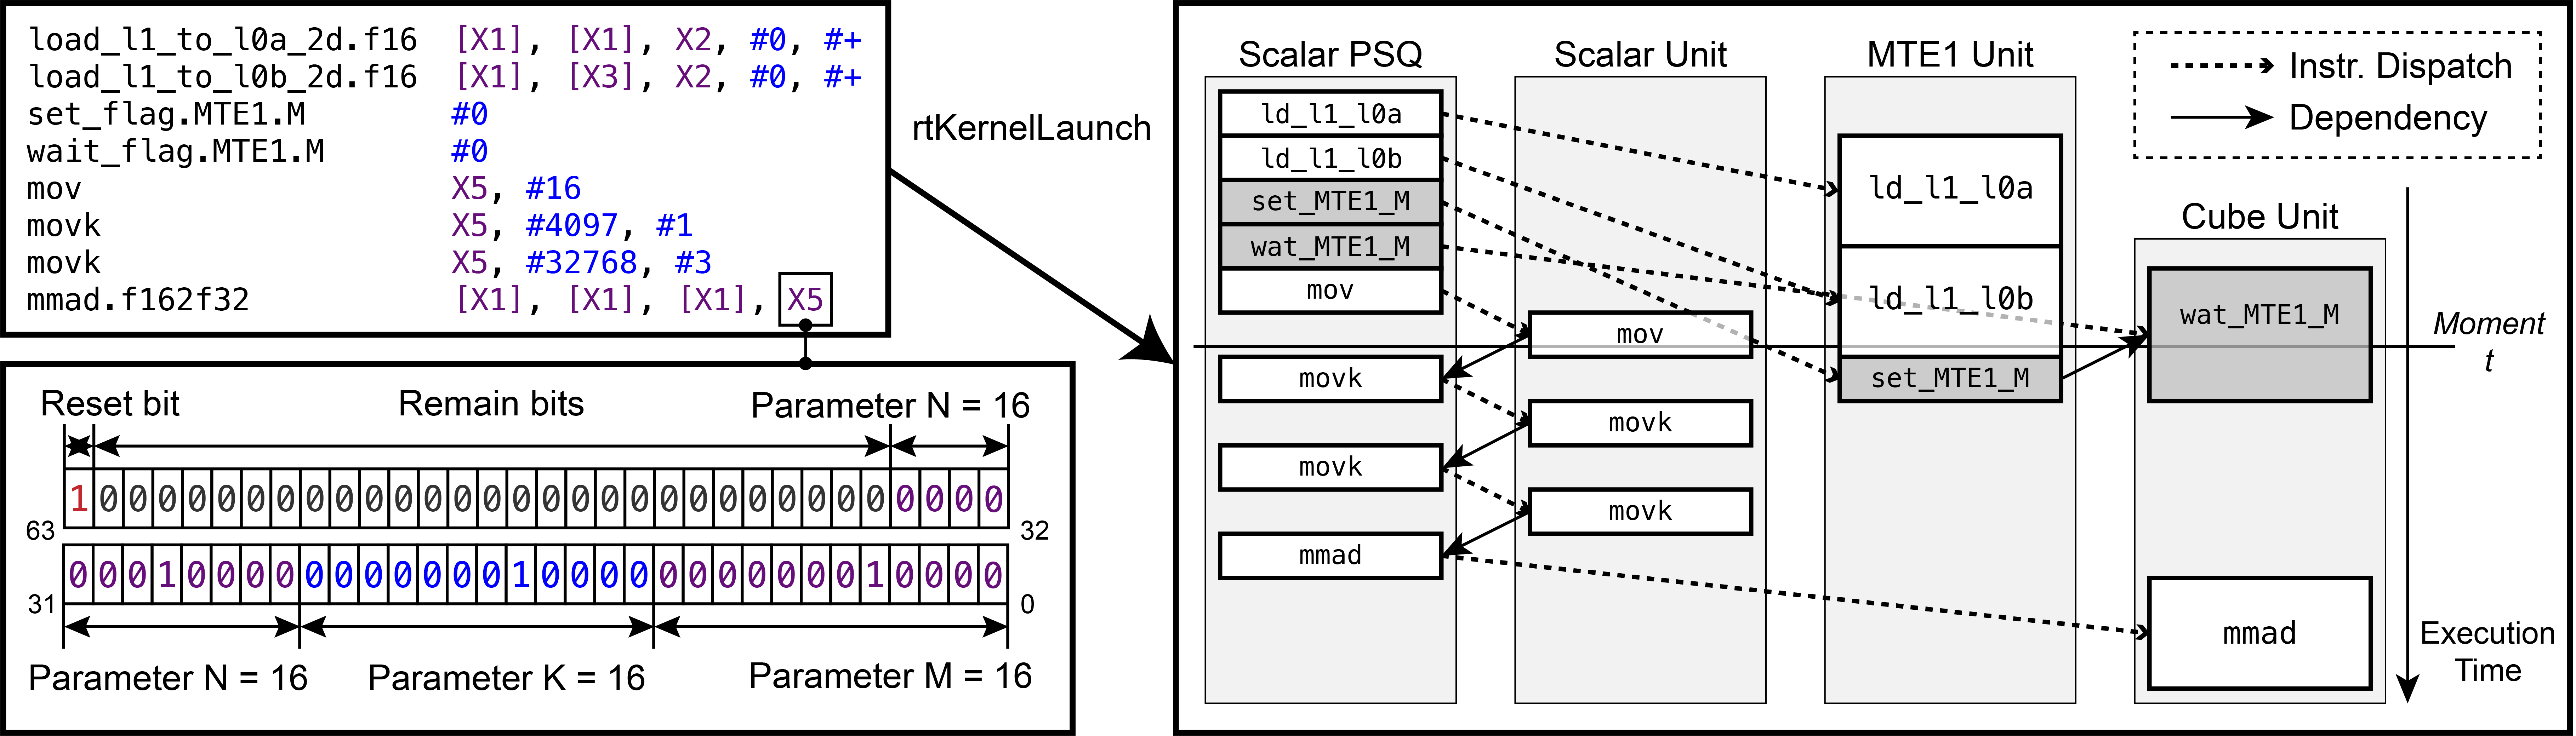
\includegraphics[scale=0.30]{figures/reduced_soft.png}
                \end{adjustbox}       
            }\\
            \centering
            \subfigure{} {
                \begin{adjustbox}{addcode={\begin{minipage}{\textheight}}
                    {\caption{The examples of kernels influenced by the binary semaphore}
                    \label{fig:instr}
                    \end{minipage}},center}
                    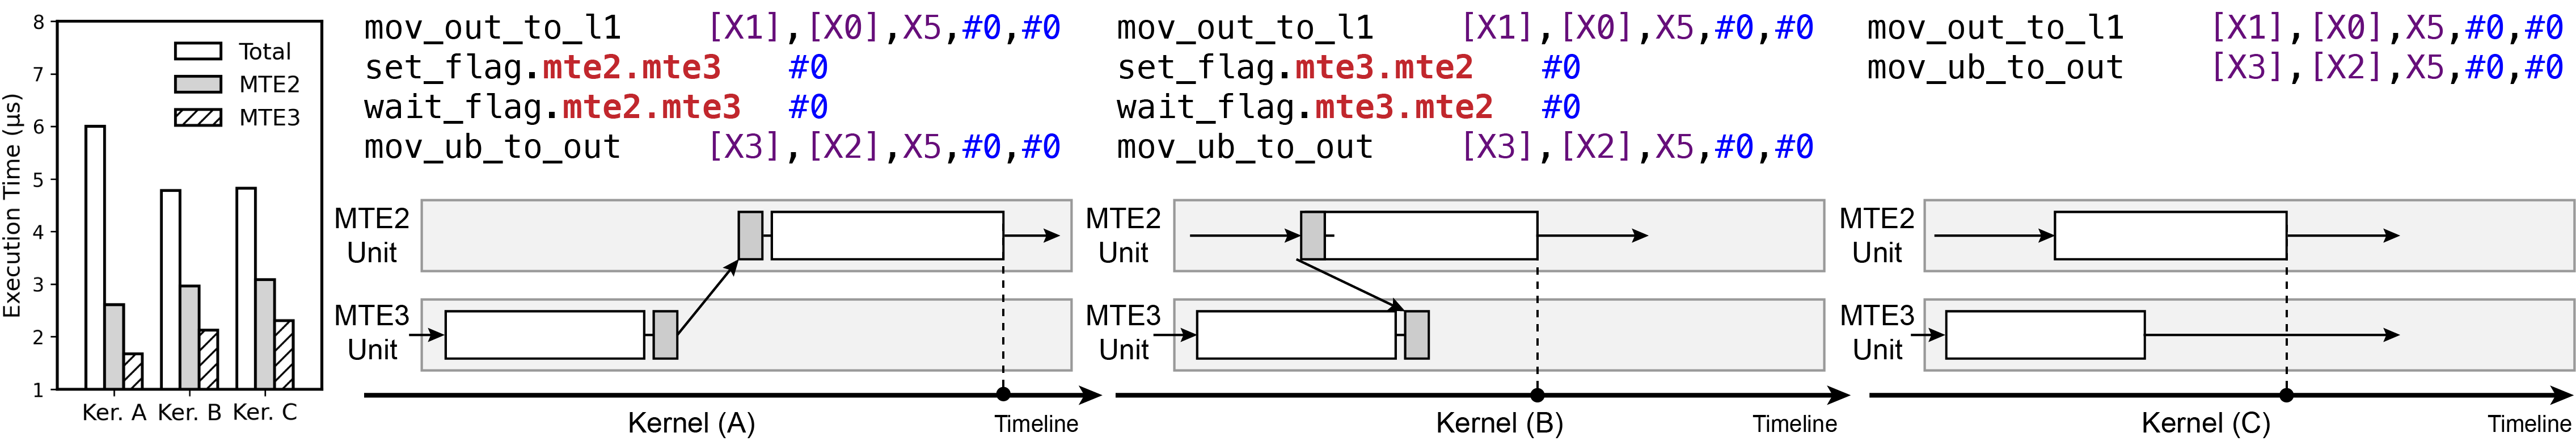
\includegraphics[scale=0.48]{figures/mov_test.png}
                \end{adjustbox}        
            }
        \end{minipage}      
    \end{adjustbox}
\end{figure}

\begin{figure}[htbp]
\end{figure}

As we demystify in Fig. \ref{fig:soft}, all the instruction queues, including the Scalar PSQ, strictly follow the FIFO policy. The Scalar PSQ maintains input kernel instructions and identifies the type of each instruction (Scalar, Vector, Cube, MTE1/2/3), which performs as Instruction Decoder in CPUs. The types of instruction determine the instruction queue to which the instruction is sent, as well as the concurrent unit on which the instruction is executed. For the Scalar instructions, the Scalar PSQ directly sends them to the Scalar Unit. For others, the Scalar PSQ sends them to the corresponding instruction queues via Instruction Dispatch. Each compute or storage unit executes one single instruction at every moment. When a unit is idle, the corresponding queue dequeues the oldest instruction to the unit for execution. The Scalar PSQ asynchronously dispatches the instructions except for the Scalar instructions.

While the DaVinci Core adopts the single-thread execution model, the concurrency of the hardware units makes the Instruction-Level Parallelism (ILP) supported. To guarantee the dependency among the units, the programmers must manually insert the \verb|set_flag| and \verb|wait_flag| instructions, acting as the binary semaphore mechanism. 
The fundamental operations of the semaphore mechanism are PV Operations \cite{EWD:EWD74}. P Operation decrements the value of the semaphore variable by 1. If the new variable is negative, it blocks the caller process. Meanwhile, V Operation increments the value of the semaphore variable by 1. If the old variable is negative, it wakes up a blocked process and lets it access a resource unit. 
In DaVinci Cores, the \verb|wait_flag| acts as P Operation and the \verb|set_flag| performs as V Operation. The Scalar PSQ assigns the two semaphore operations to the corresponding instruction queue just as it does with other instructions. In the example of the moment \verb|t|, following the FIFO policy, the \verb|set_flag| (\verb|set_MTE1_M|) in the MTE1 queue shall not start due to the incompleteness of the last instruction \verb|ld_l1_l0b|. The corresponding \verb|wait_flag| (\verb|wat_MTE1_M|) keeps blocking the Cube Unit until the execution of \verb|set_flag|. Therefore, the instruction \verb|mmad| shall not start before the end of the \verb|ld_l1_l0b|.

\begin{figure}[htbp]

\end{figure}

The idleness of the hardware unit caused by the synchronization is one of the most critical factors influencing the execution time. Each instruction could prolong or block the execution based on its programming logic. Furthermore, the concurrent execution can be intentionally activated or deactivated, which is decided by how the kernel programs schedule the multiple semaphore registers and control flows. Fig. \ref{fig:instr} illustrates a simple DaVinci kernel containing two data transfer operations (on MTE2 and MTE3 Units) with different binary semaphore operations. As a result, Kernel (A) takes 1.26$\times$ more time than Kernel (B) and 1.24$\times$ more than Kernel (C), while the actual two data transfer operations take similar time among all kernels. 
For Kernel (A) and Kernel (B), the parameter order (\verb|mte2.mte3| \& \verb|mte3.mte2|) of the semaphore operations determines the execution time. The parameter order \verb|mte2.mte3| prohibits the concurrent execution while the reversed \verb|mte3.mte2| does not, which reports a similar result to Kernel (C).
Therefore, the DaVinci Core working details make the modeling methods based on kernel metadata analysis or statistics ineffective, e.g., the most straightforward execution time computed by $DataSize / Bandwidth$. From the view of those modeling methods without analysis in the instruction logic, Kernel (A) and (B) should have a similar total execution time, which is false in our evaluations. Then it is necessary to model the performance with the instruction-level analyses in the kernel source codes.

\subsection{Overview of Verrocchio}

\begin{figure}[htbp]
    \begin{adjustbox}{addcode={
        \begin{minipage}{\width}}{
            \caption{Verrocchio, a discrete-event-based performance model}
            \label{fig:over}
        \end{minipage}},rotate=90,center}
        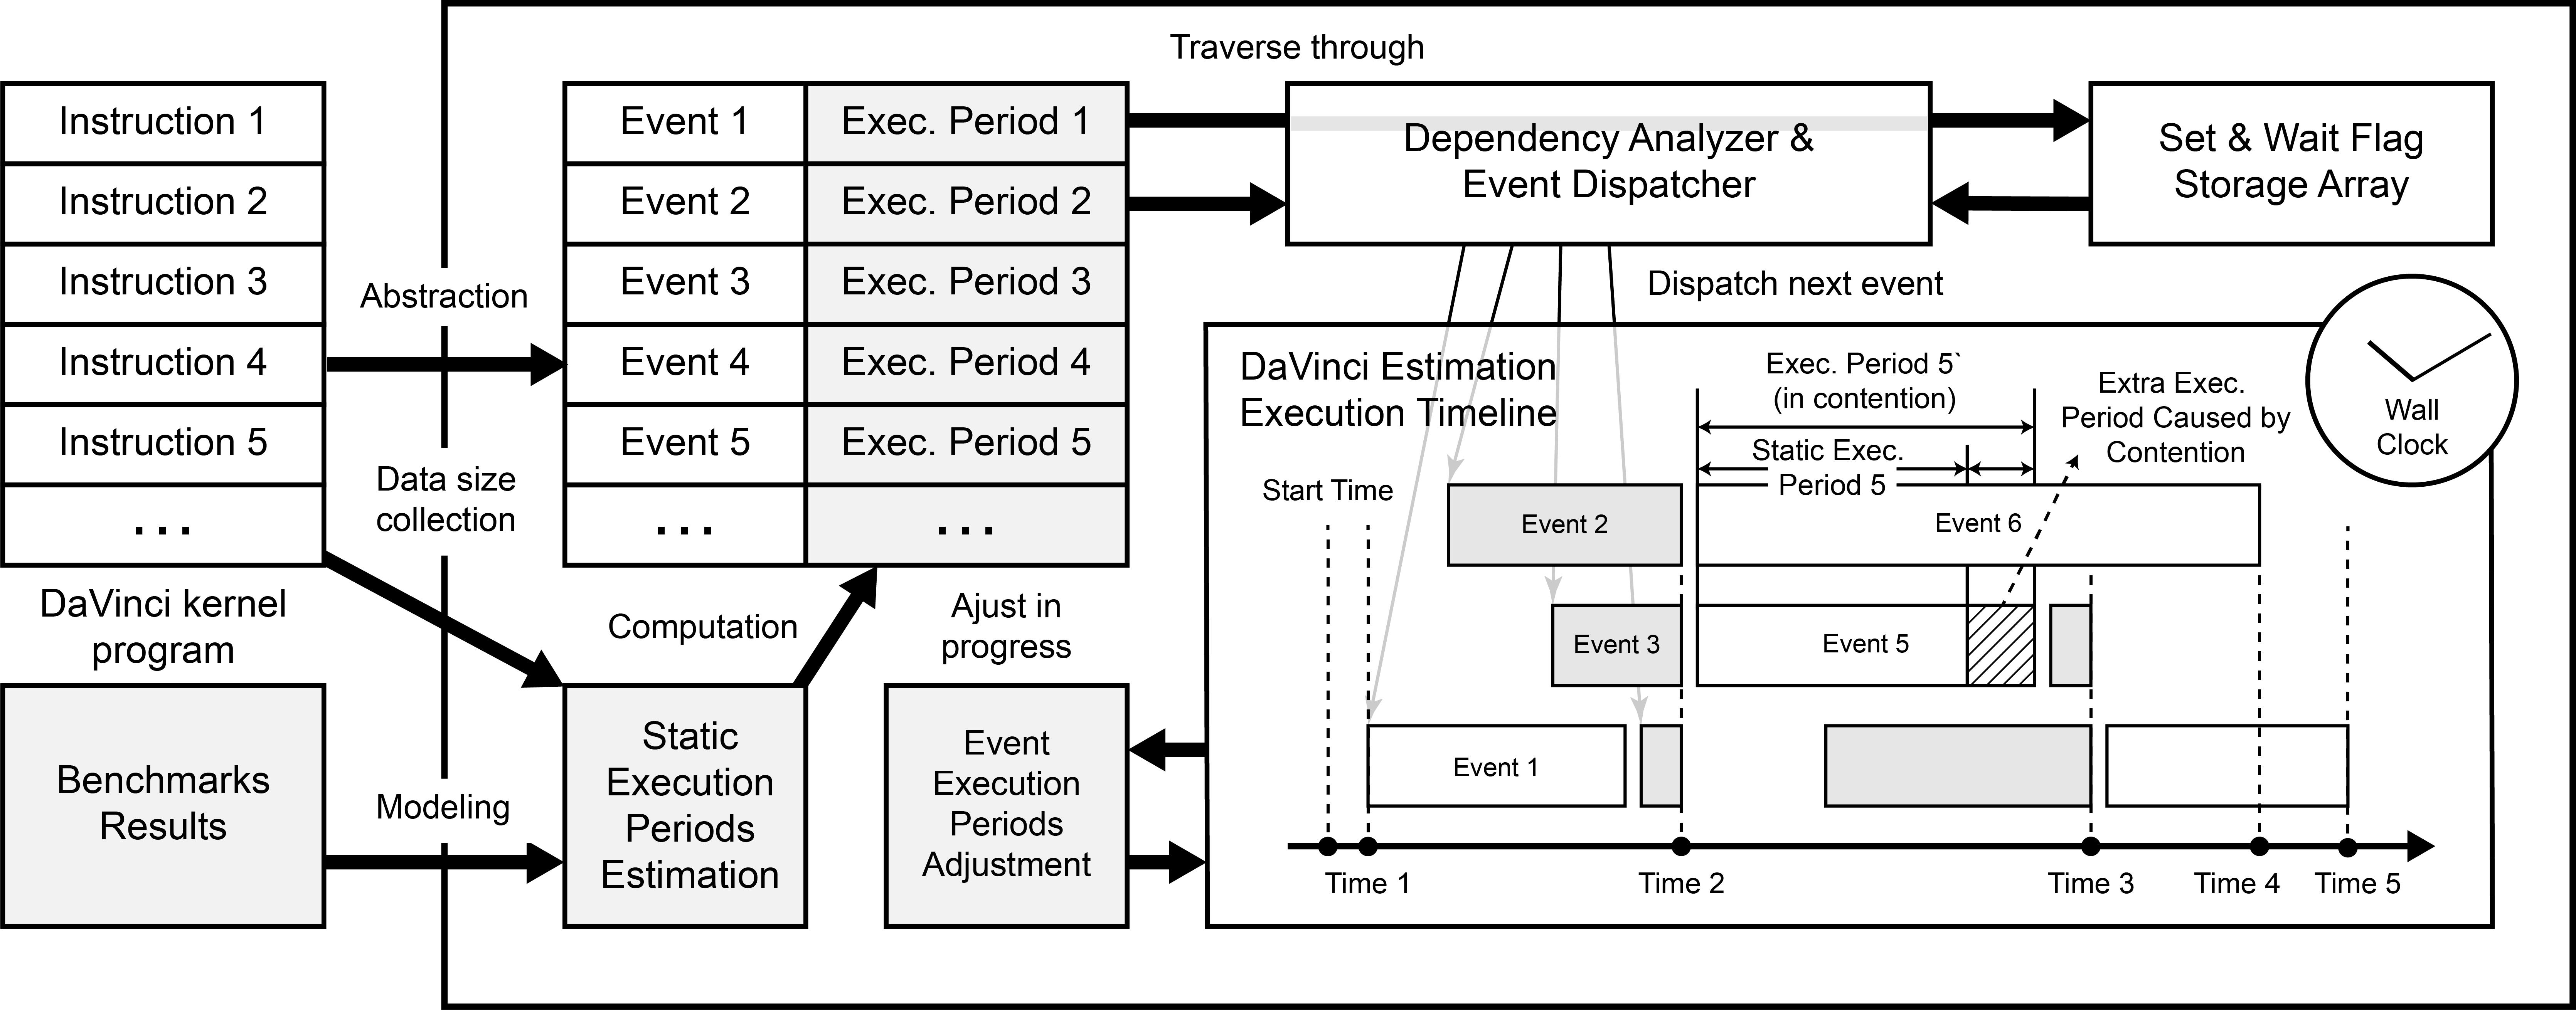
\includegraphics[scale=0.33]{figures/overview.png}
    \end{adjustbox}
\end{figure}

Verrocchio is a discrete-event-based performance model, where events occur due to occurrence time with execution periods at the discrete points in time. Fig. \ref{fig:over} illustrates the structure of our DaVinci Core model. Verrocchio has two inputs, the target program source codes and the hardware benchmark results. It predicts and outputs the execution period of the kernel program.

To provide instruction-level modeling for the kernel program, Verrocchio first scans the instructions of the kernel program to abstract them into discrete events. It also collects the data size for each instruction. Verrocchio applies the results from our instruction-level micro-benchmarks, which target to expose the hardware performance, especially the DaVinci Core storage unit performance. Combining the data size and the benchmark results, Verrocchio estimates the static execution period of each instruction, which is the execution period when the instruction executes alone.

Two core components of Verrocchio are the dependency analyzer and event dispatcher, which manage the prepared discrete events and place them on a DaVinci execution timeline at the correct timestamp with a wall clock. To handle the synchronization supported by the binary semaphore, Verrocchio maintains two arrays from the analysis of the prepared events. The two sorted arrays store the Set Flag and Wait Flag operations and guide Verrocchio correctly start an event when meeting the binary semaphore conditions. As we discussed, during the procedure, the event execution periods can be updated because of the bandwidth contention, as the example of Event 5 shown in Fig. \ref{fig:over}. To model the contentions, Verrocchio offers the execution periods adjustment, which updates the new execution periods each time the contentions begin and end.

\section{Benchmarking DaVinci}

To reveal the performance of the storage unit, we benchmark the Ascend 310 processor by launching a series of instruction-level micro-benchmarks. For the hardware units, whose performance reports a regular and stable trend, the benchmark increases the processed data size and computes the bandwidth by the least-square method. For the bus bandwidth, which connects to the external storage and involves the contention by the MTE2 and MTE3 Units, we first design a specifically-crafted benchmark to identify the contention source and expose the runtime behaviors. Then we adopt further benchmarks with different contention ratios to quantify the bandwidth sharing under contentions.

\subsection{Benchmarks for Hardware Units \label{sec:cube_bench}}

\subsubsection{Methodology}

For the MTE1 Unit, we directly adopt the micro-benchmark kernels. For the Vector Unit, we list the data movement bandwidth here and with a precision converting function from FP32 to FP16. For the Cube Unit, we benchmark the FLOPS by modifying the \verb|mmad| instruction parameters. The computation amount of each minimized $16 \times 16 \times 16$ matrix multiplication is $(15 + 16) \times (16 \times 16) = 7936$ FLOPs. After the single-core benchmarks, we activate and benchmark two DaVinci Cores on the Ascend 310 processor. We compare the results with the single-core results to check whether the double-core execution can approximately double the bandwidths or FLOPSs. In addition, we also benchmark the kernel launch time of double-core execution compared with the single-core execution. 

\subsubsection{Benchmark Results} 

\begin{table}[tbp]
    \caption{Ascend 310 Cube Unit benchmark results}
    \label{tab:bench}
    \begin{center}
    \scalebox{0.73}{
        \begin{tabular}{c|c|c|c}
        \toprule[1pt]
        \textbf{Benchmark Types} & \textbf{Double-Core} & \textbf{Single-Core} & \textbf{Percentages} \\
        \midrule[0.5pt]
        MTE1 bw. (L1 Buffer to L0A Buffer) & 695.97 GB/s & 347.99 GB/s & 99.99\% \\
        MTE1 bw. (L1 Buffer to L0B Buffer) & 348.79 GB/s & 174.37 GB/s & 100.00\% \\
        Vector bw. (None) & 348.16 GB/s & 174.06 GB/s & 100.00\% \\
        Vector bw. (F32 to F16) & 348.2 GB/s & 174.09 GB/s & 100.00\% \\
        \midrule[0.5pt]
        Cube Unit practical FLOPS (RESET off) & 10796.92 GFLOPS & 5390.32 GFLOPS & 100.00\% \\
        Cube Unit practical FLOPS (RESET on) & 10789.17 GFLOPS & 5397.34 GFLOPS & 99.99\% \\
        Ascend 310 documented FLOPS & - & 4096.00 GFLOPS & - \\
        \midrule[0.5pt]
        Kernel launch time & 2293.5 ns & 2354.5 ns & - \\
        \bottomrule[1pt]
        \end{tabular}
    }
    \end{center}
    \end{table}


We list the benchmark results in Table \ref{tab:bench}. We summarize two main observations of the results as follows:

\begin{itemize}
    \item As we expected, the independent hardware units report perfectly double acceleration. These hardware units require on-core resources only (bandwidths and computation power) and shall not suffer performance loss in the multi-core execution situation because of the Interconnect Bus.
    
    \item The kernel launch time results report that the double-core execution shows no apparent kernel launch time extension compared with the single-core execution. We assert that the kernel launch time does not suffer from any contentions in double-core execution. As DaVinci Cores have no inter-core communication mechanism, we assume that the two DaVinci Cores on Ascend 310 processors start and execute the kernel synchronically.
\end{itemize}


\subsection{Benchmarks for Bus Contention Source and Runtime Behaviors}

While the bandwidth of the individual bus execution can be evaluated naturally with the benchmark in Sec. \ref{sec:cube_bench}, the contention caused by the multiple units is non-trivial to be measured. In this subsection, we design a benchmark to study the source and the runtime behaviors of the contentions observed at the DaVinci Cores bus, which are caused by the MTE2 and MTE3 Units. 

\subsubsection{Benchmark Design \label{sec:ben_des}}

\begin{figure}[tbp]
    \centering{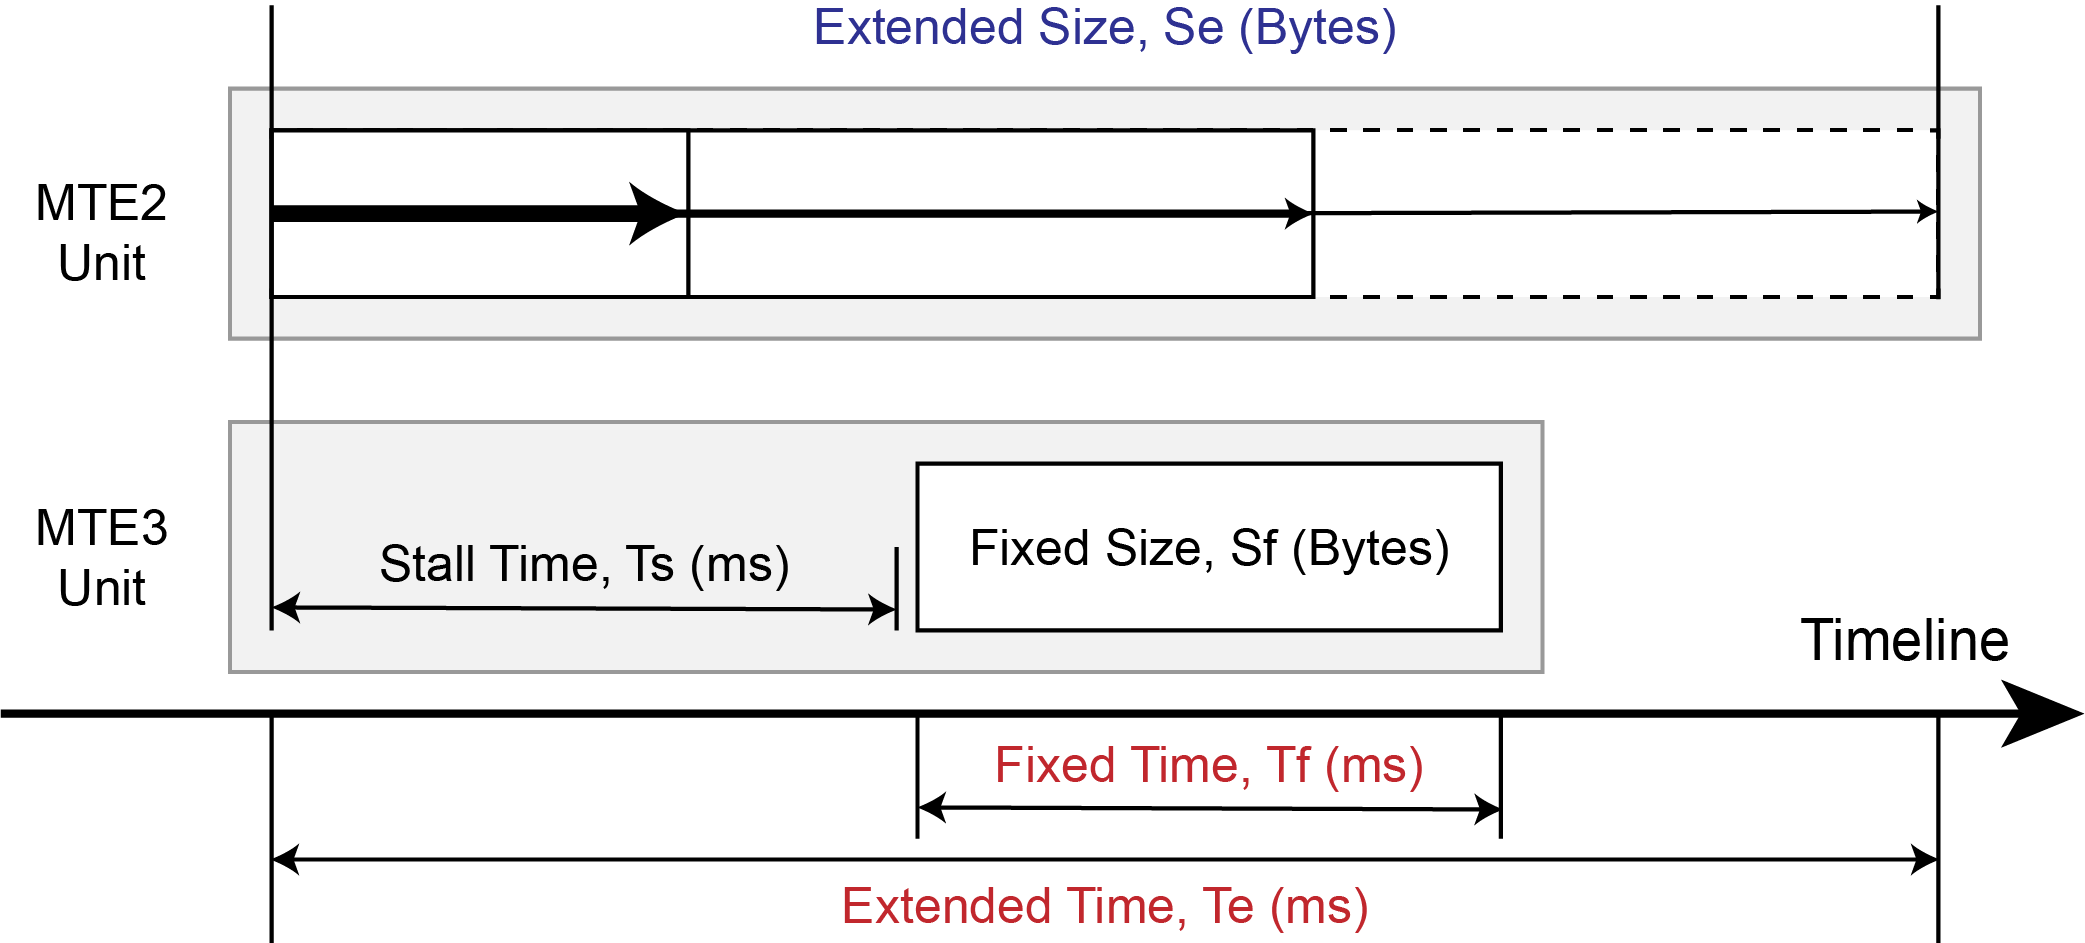
\includegraphics[scale=0.55]{figures/bench_meth.png}}
    \caption{Bandwidth contention monitoring benchmark (e.g., MTE2 \& MTE3 Units)}
    \label{fig:bench_meth}
    \end{figure}


\begin{algorithm}[tbp]
    \caption{Bandwidth Contention (e.g., MTE2 \& MTE3 Units)}
    \label{alg:bench_meth}
        
    \SetKwInOut{Input}{input}
    \SetKwInOut{Output}{output}
        
    \BlankLine
    \Input{
        Stall time, $T_{s}$; Fixed size, $S_{f}$
    }
            
    \Output{
        Extended time array: $A_{e}$; Fixed time array: $A_{f}$
    }
    \BlankLine

    \For{$Se : 0 \to $ MAX}{
        \textbf{Barrier call} \\
        \textbf{(MTE2)} Process data of size $S_{e}$ \\
        \textbf{(Scalar)} Dummy instruction \\
        \textbf{(Scalar)} $\cdots$ $\cdots$ \  (Block instruction 7 for $T_{s}$)\\
        \textbf{(Scalar)} Dummy instruction \\
        \textbf{(MTE3)} Process data of size $S_{f}$ \\
    }
\end{algorithm}

The objective of the benchmark is to monitor the behaviors of the entire contention runtime, from the start to the end of it, with a fixed contention ratio of two (the MTE2 and MTE3 Units). 
As shown in Fig. \ref{fig:bench_meth},
on one of the hardware units (e.g., the MTE2 Unit), we first let the unit process an increasing size of data, $S_{e}$, and then keep it idle until the end. For the other hardware unit (e.g., the MTE3 Unit), which is concurrently executing alongside, it first stays idle for a short period $T_{s}$ and then processes a segment of data with the size of $S_{f}$ until the end. 
On the DaVinci Cores, we insert dummy Scalar instructions between the instructions of the former unit and the latter, as annotated in Alg. \ref{alg:bench_meth}. 
As discussed, the Scalar PSQ must wait until the end of the Scalar instructions and proceed to the next instruction. Therefore, the dummy instructions block the Scalar PSQ and keep the latter unit idle. When the former unit has been executing for a period, the latter unit finally receives its instruction from the Scalar PSQ and then executes with the designed contention. We measure and record the execution time of two units, $T_{e}$ and $T_{f}$ with the Huawei official profiler respectively, with the increment of $S_{e}$.

Divided by $T_{e}$, the two hardware units experience three contention statuses: before, under, and after contention. When $T_{e} < T_{s}$, where $S_{e}$ is not large enough, the two hardware units stay the status before contention. When $T_{e} < T_{s} + T_{f}$, the two units are under contention. When $T_{e} > T_{s} + T_{f}$, the two units finish the contention periods at the status after contention. Therefore, after finishing the benchmark in Alg. \ref{alg:bench_meth}, the recorded execution time $T_{e}$ and $T_{f}$ can expose the entire runtime behaviors during the bandwidth contention. In addition, we vary the input parameters $T_{s}$ and $S_{f}$ to study the potential influences by the contention beginning time and processed data size under contention.

\subsubsection{Contention Source and Runtime Behavior Results \label{sec:runtime}}

\begin{figure}[t]
    \centering{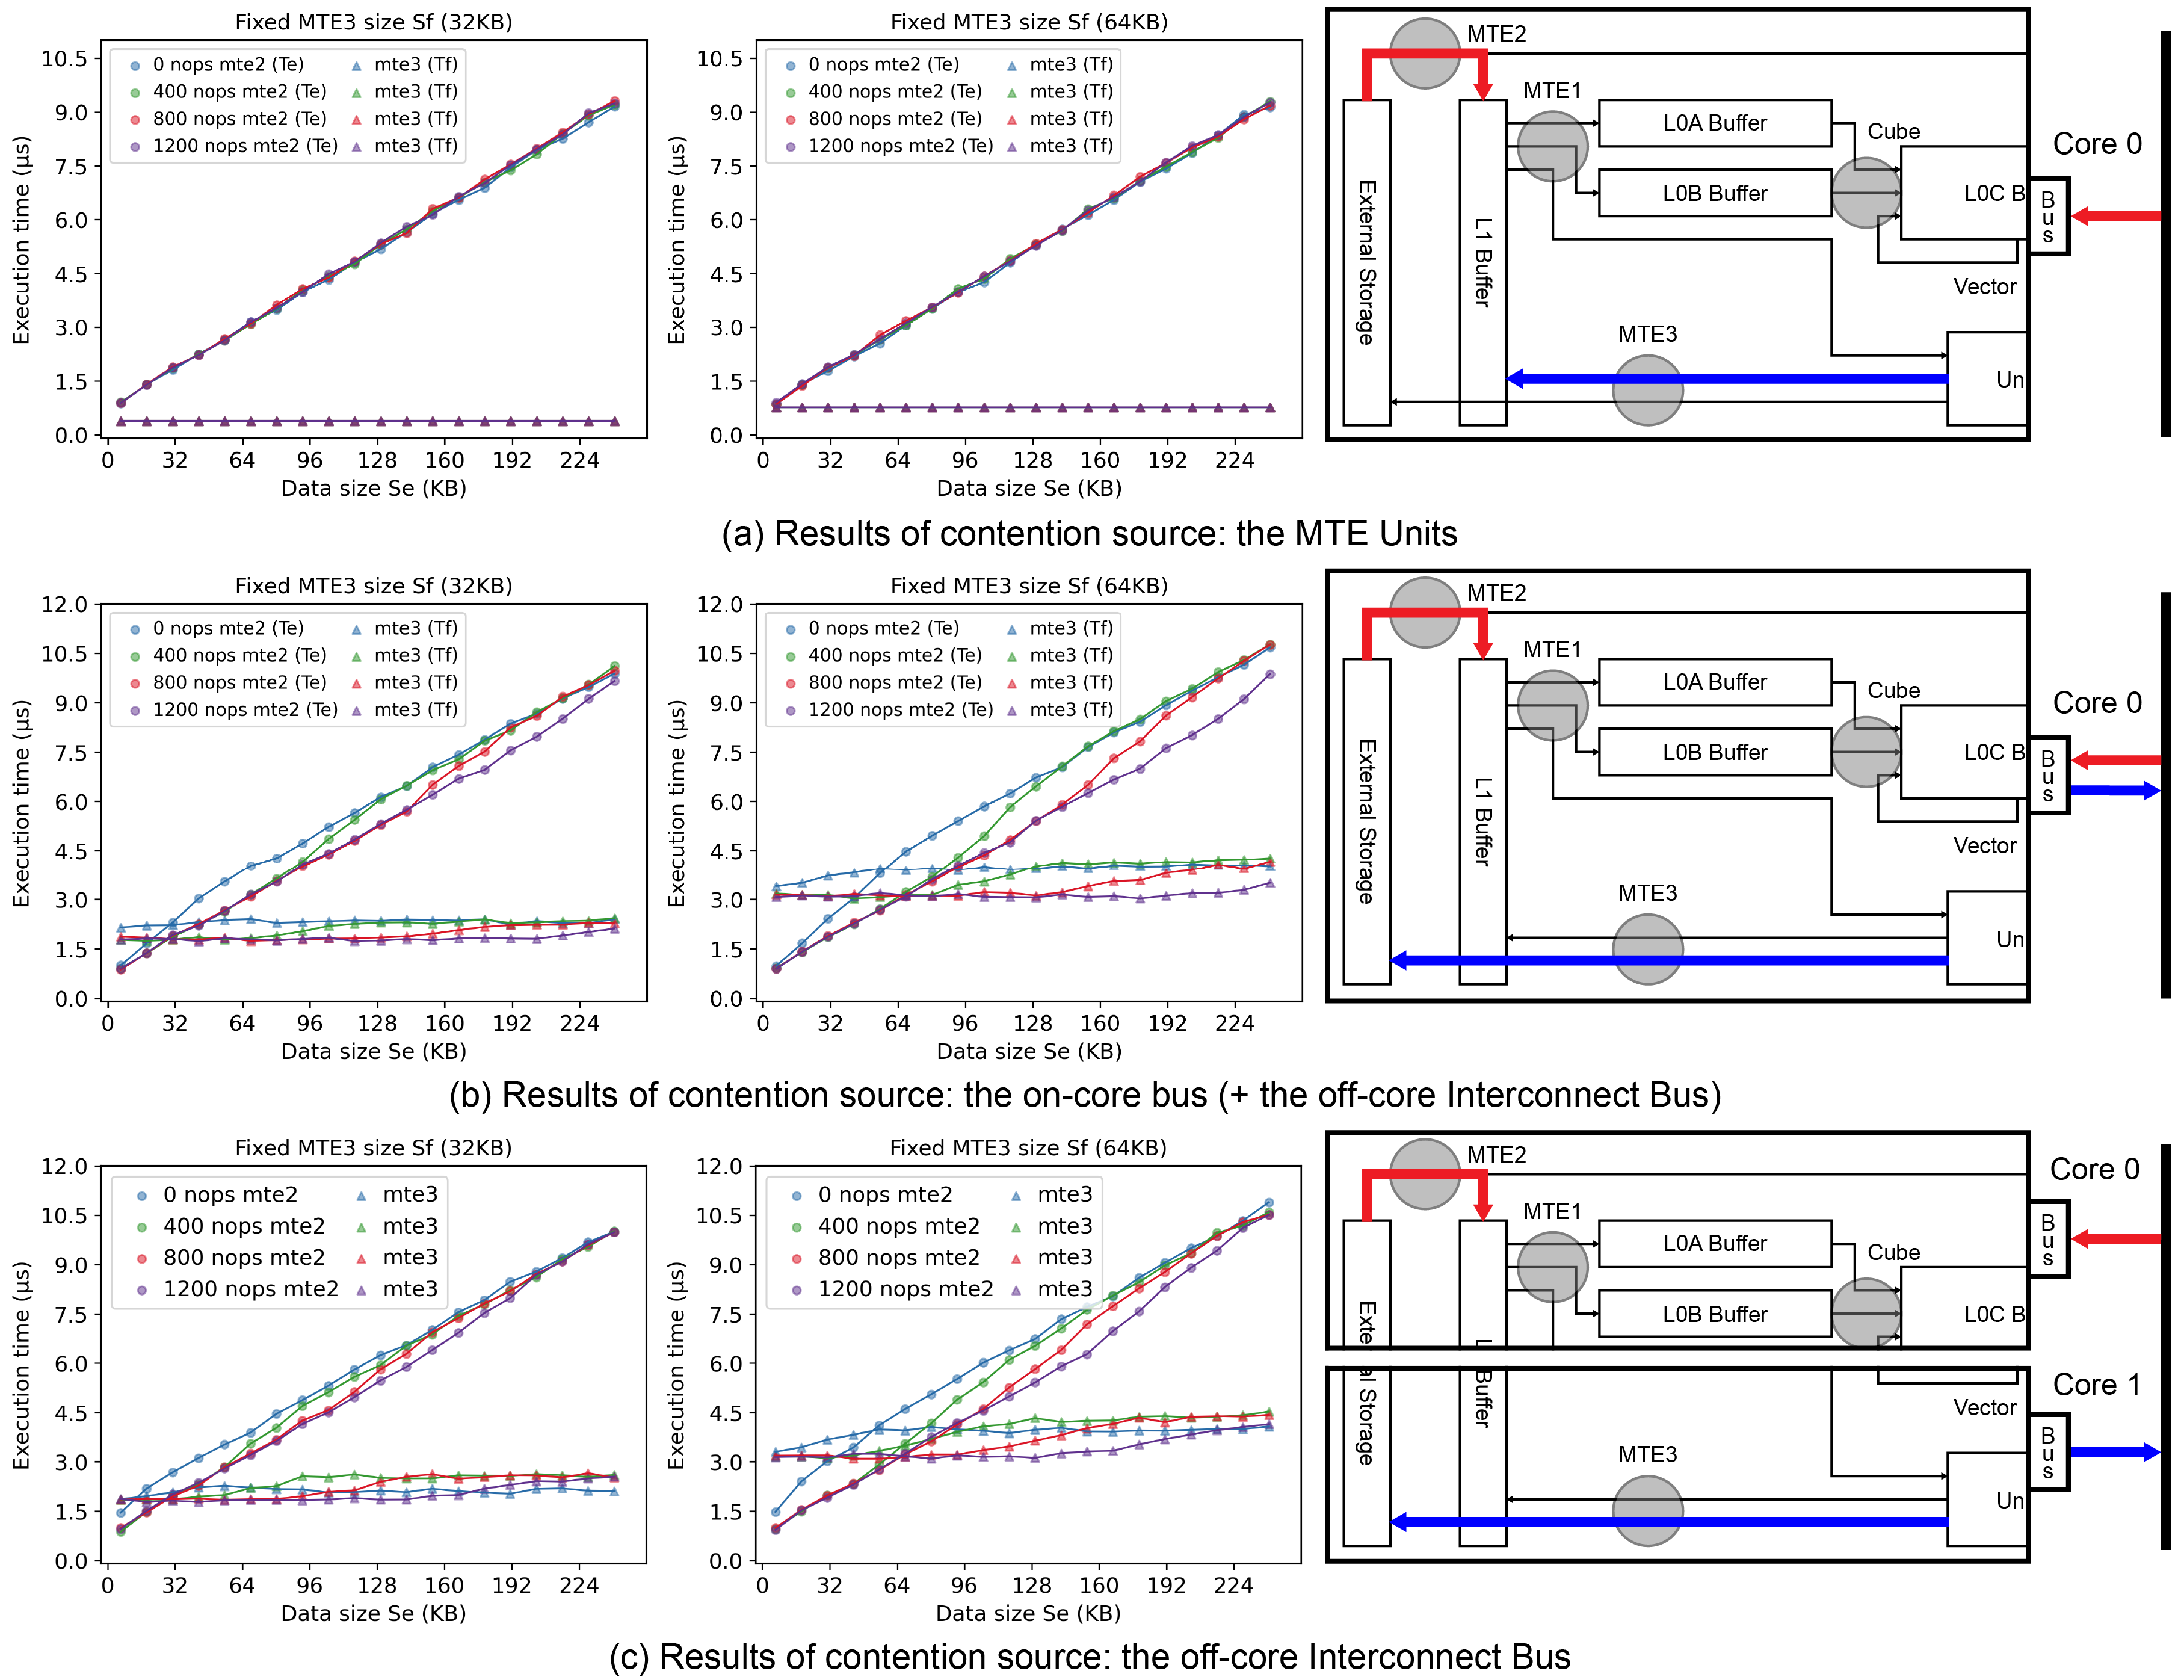
\includegraphics[scale=0.43]{figures/cont_source.png}}
    \caption{Contention source results with the corresponding data paths}
    \label{fig:cont_source}
    \end{figure}

Based on the fundamental benchmark designed in Sec. \ref{sec:ben_des}, we illustrate the benchmark results of the MTE2 and MTE3 Units with the different corresponding data paths in Fig. \ref{fig:cont_source}. We insert NOP instructions as dummy instructions, the number of which (related to $T_s$) are annotated in the legend of figures.

We first call the instructions for transferring data between the external storage and the L1 Buffer (MTE2) and that between the Unified Buffer and L1 Buffer (MTE3) concurrently, which does not involve other data paths. The results in Fig. \ref{fig:cont_source} (a) show that with the variation of $S_f$, $S_e$, and $T_s$, the evaluated execution time $T_f$ and $T_e$ remain unchanged, which indicates no contention happens between the two MTE Units.

By contrast, from the results in Fig. \ref{fig:cont_source} (b) and (c), we observe apparent irregular execution time variations, which present clear bandwidth contention runtime behaviors. For both the MTE2 and MTE3 Units, it is easy to identify the turning points of the three contention statuses we described in Sec. \ref{sec:ben_des}. With the increment of the data size $S_e$, the MTE2 Units report two different slopes in three-segment polylines, where the first segment is before contention, the second is under contention, and the third is after contention. For the MTE3 Units with a fixed data size $S_f$, which were supposed to take a stable execution time, the contentions bring an extra execution time increment and also result in three-segment polylines. The number of the NOP instructions determines $T_s$ and the length of the first segment. The increment of the MTE3 fixed data size $S_f$ extends the second segment, which shows a lower bandwidth because of the sharing of the limited bandwidth under contention. The third segment's slopes are the same as the first for both the MTE2 and MTE3 Units, indicating that the bandwidths recover from the contention without extra side effects.

For the contention source, since it is impracticable to transfer the data without the off-core Interconnect Bus independently, the results shown in Fig. \ref{fig:cont_source} (b) are introduced by both the on-core buses and the off-core Interconnect Bus. Meanwhile, Fig. \ref{fig:cont_source} (c) involves the off-core Interconnect Bus only by placing the two instructions on two DaVinci Cores separately. In this way, in Fig. \ref{fig:cont_source} (c), the on-core bus of Core 0 transfers data to the DaVinci Core with the MTE2 Unit individually and avoid any possibilities for contentions. Comparing the results of Fig. \ref{fig:cont_source} (b) and (c), the execution time, the variation trends, and the slopes are similar, which suggests they activate the same contention source. Therefore, we assert that the contention source of the Ascend 310 processor bus bandwidth is the common part of Fig. \ref{fig:cont_source} (b) and (c), the off-core Interconnect Bus.

\begin{figure}[tbp]
    \centering{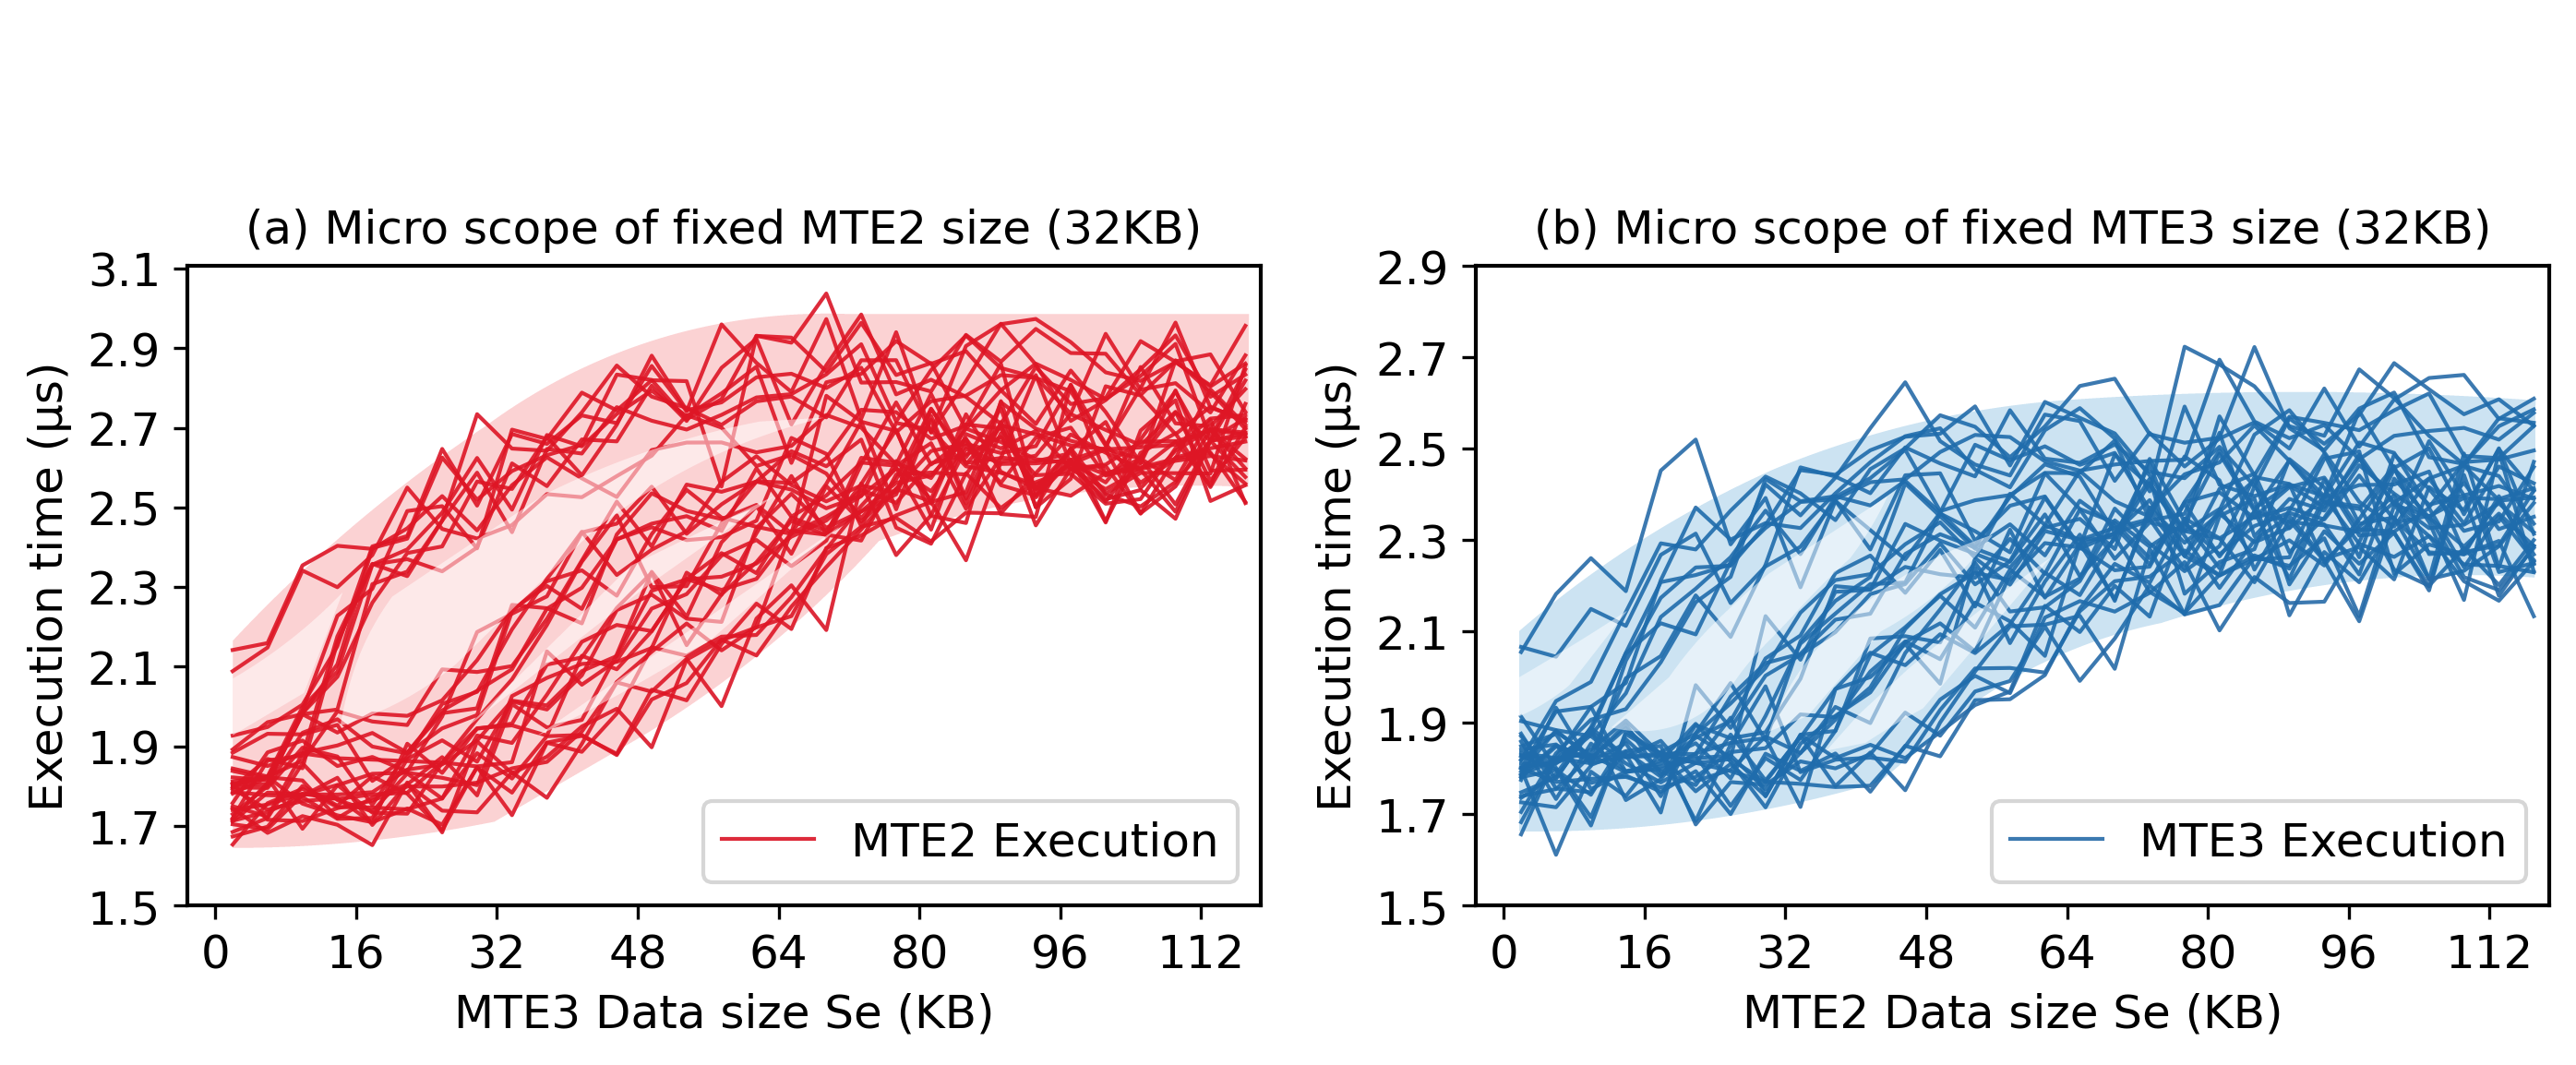
\includegraphics[scale=0.53]{figures/micro_view.png}}
    \caption{The execution of the MTE Units with tiny $T_{s}$ increments}
    \label{fig:micro_view}
    \end{figure}

Fig. \ref{fig:micro_view} shows the results of the second benchmark, where we repeat the benchmark shown in Fig. \ref{fig:cont_source} (b) but increase $T_{s}$ with tiny steps to explore the execution patterns of the MTE Units under contention. Fig. \ref{fig:micro_view} (a) plots the fixed-sized MTE2 Unit execution results ($S_f$ = 32 KB) with the increasing MTE3 Unit data size $S_e$ while Fig. \ref{fig:micro_view} (b) is symmetric. With the increment of $T_{s}$, the beginning of the contention delays, which increases the start points of the second segment we discuss in Sec. \ref{sec:ben_des} accordingly. However, from the results for the two cases, we observe that although $T_{s}$ grows evenly, the start points of the second segments are not averagely distributed along the x-axis but gather at specific points, especially for the MTE3 Unit. The execution patterns show that the MTE Unit does not start the data transfer and forms a contention instantly after execution, suggesting the data is transferred in blocks or segments. We assert that before block transferring, the Interconnect Bus must manage and decide how to share the bandwidth based on the number of executing Units each time.

\subsection{Benchmarks for Bandwidth Sharing under Contention}

After identifying the contention source and runtime behaviors, the maximum contention ratio ($R_{max} = 4$) and the participated hardware units (the MTE2 \& MTE3 Units on two DaVinci Cores) are also determined. We further analyze the detailed policy for the potential participants to share the bandwidth. 

\begin{figure}[tbp]
    \centering{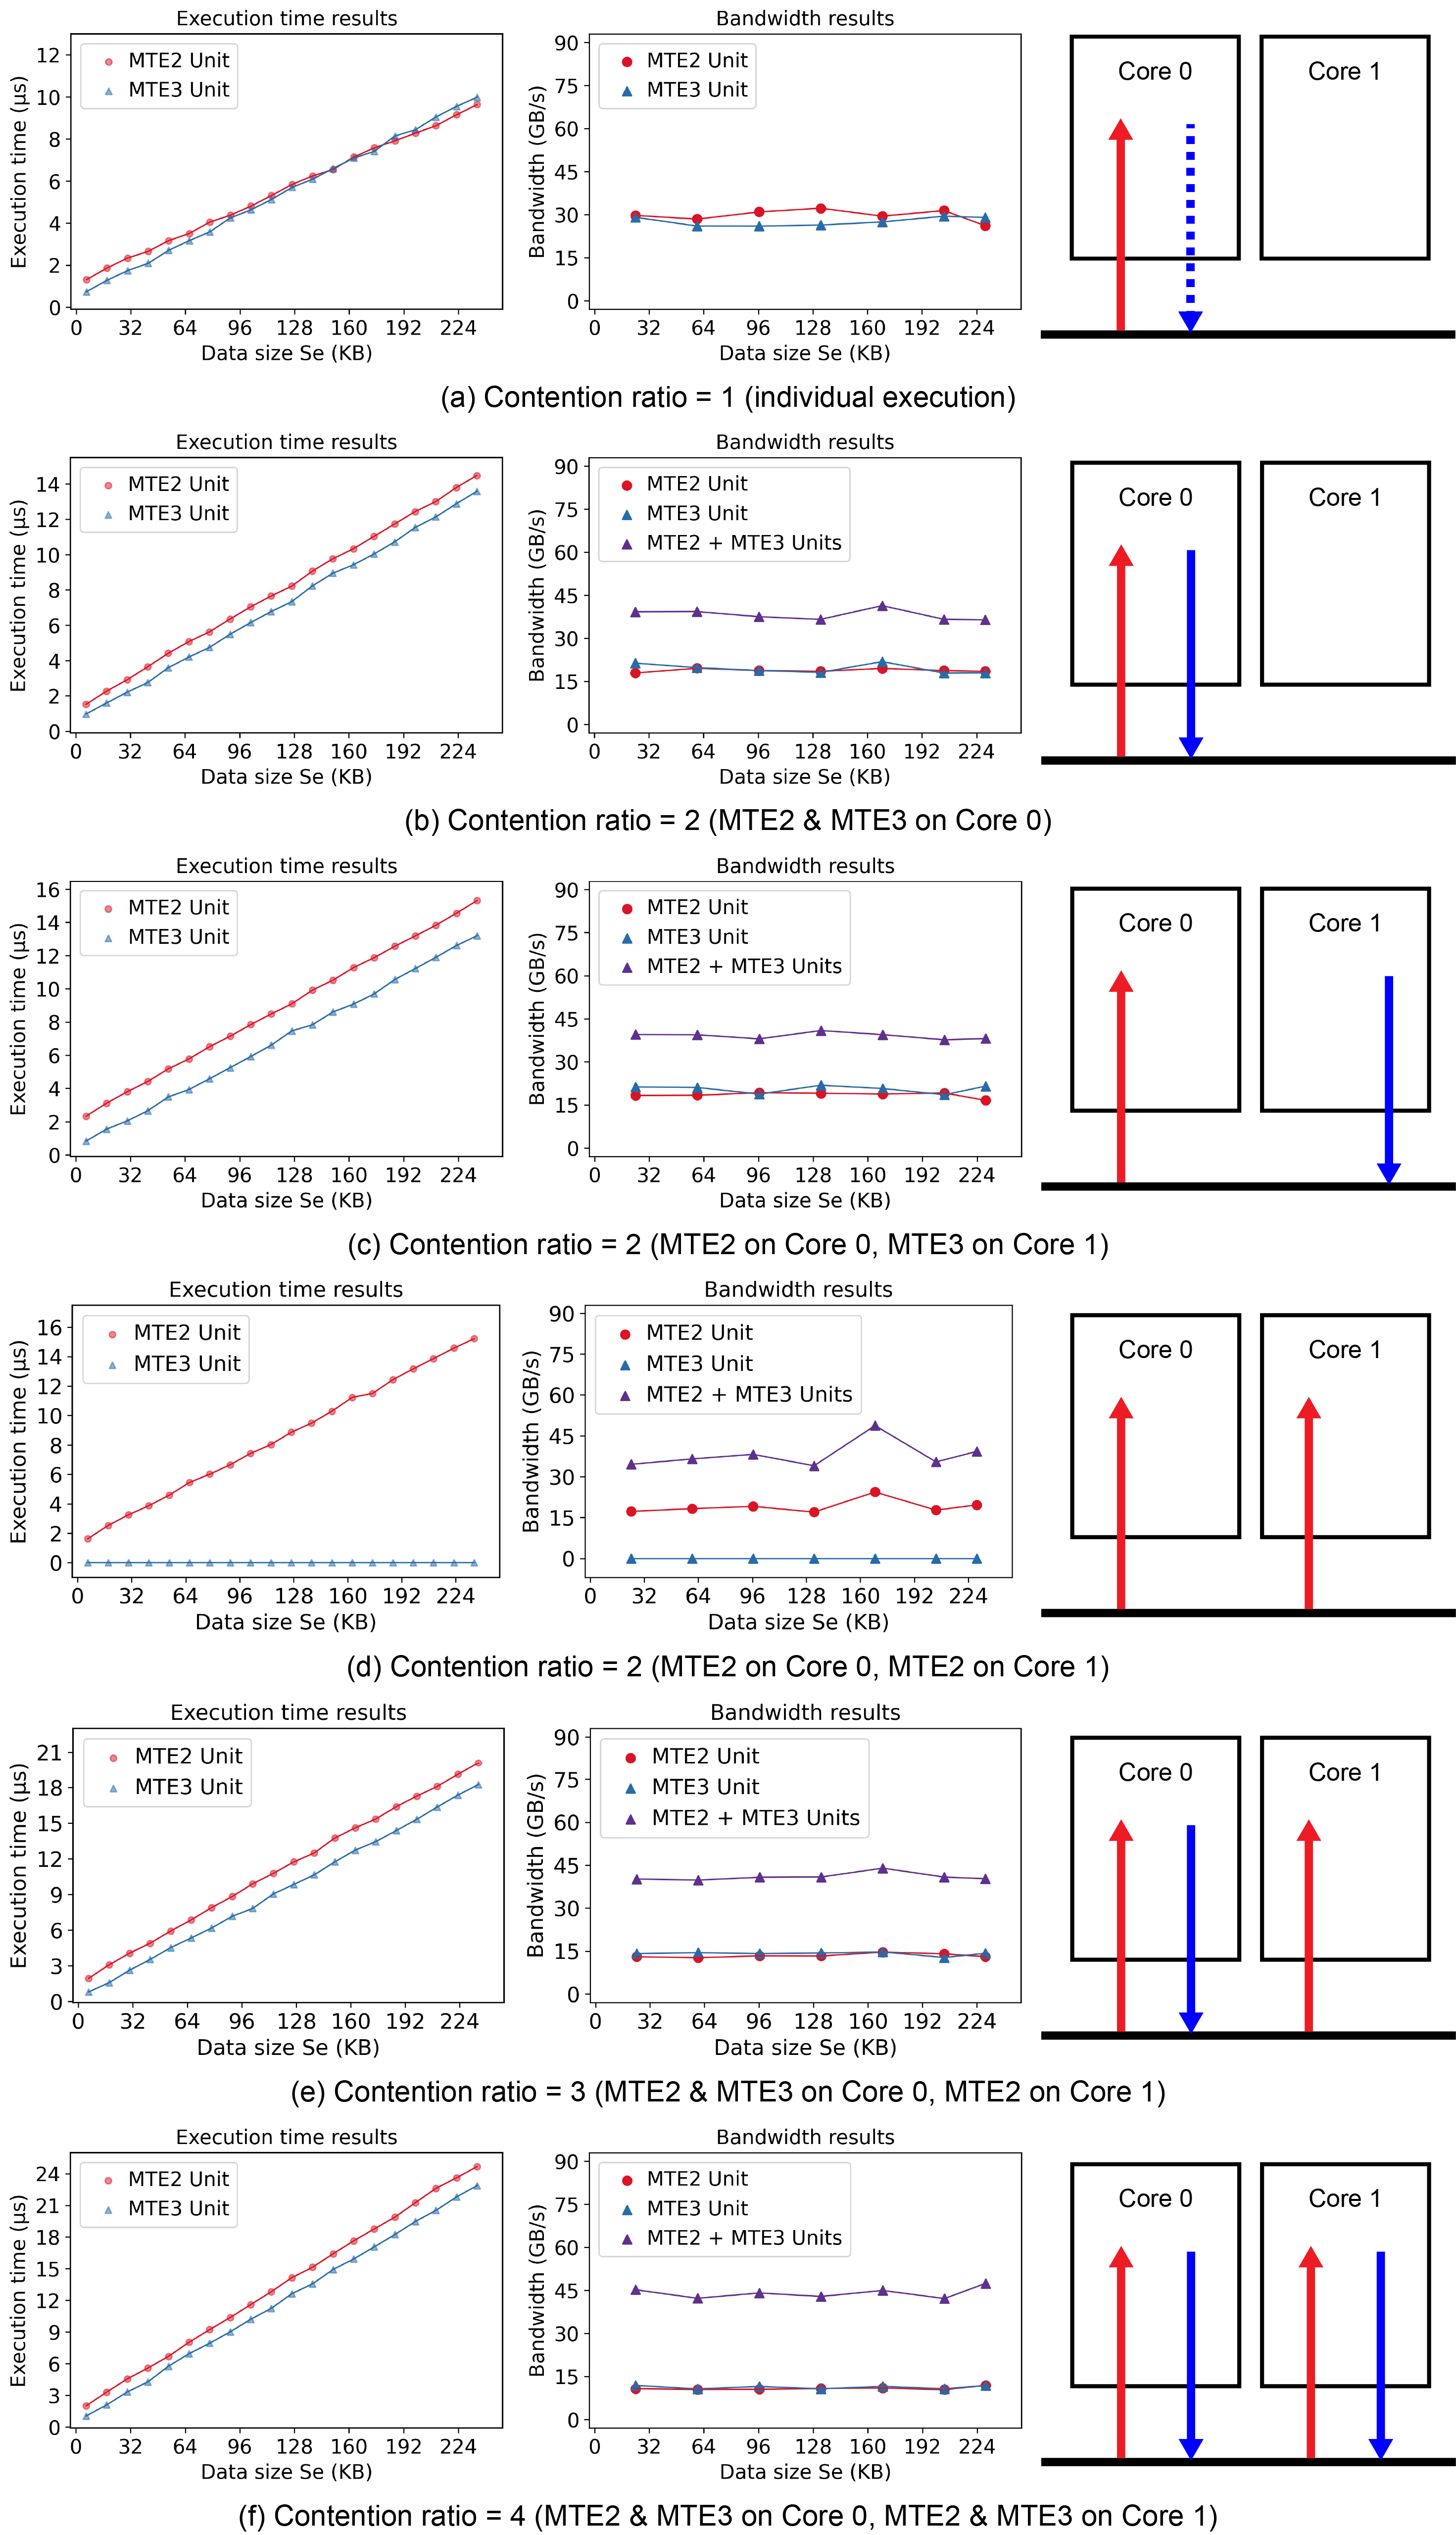
\includegraphics[scale=0.42]{figures/bw_sharing.png}}
    \caption{Bandwidth sharing of the Ascend 310 processors under contention}
    \label{fig:bw_sharing}
    \end{figure}

\subsubsection{Methodology}

We follow the benchmark used in Sec. \ref{sec:cube_bench}, where we increase the processed data sizes and compute the bandwidths under contention using the least-square method. We control the active hardware units, which are involved in the contentions of each case, with different instructions on two DaVinci Cores, respectively. Especially for the MTE3 Units, the benchmarks transfer the data from the Unified Buffer to the external storage, similar to Fig. \ref{fig:cont_source} (b).

\subsubsection{Bandwidth Sharing Results \label{sec:bw_sr_res}}

Fig. \ref{fig:bw_sharing} illustrates the benchmark results for six cases, which include all potential cases under contention. The bandwidth result of each MTE Unit plotted in the chart is the bandwidth of a single operation. Therefore, for the example in Fig. \ref{fig:bw_sharing} (e), the total bandwidth is computed by $2 \times bw_{MTE2} + bw_{MTE3}$. Generally, with the increment of the contention ratio, the total bandwidth (MTE2 $+$ MTE3 Units) also grows with a maximum bandwidth of about 42 GB/s when the contention ratio is 4, shown in Fig. \ref{fig:bw_sharing} (f). 

The bandwidths of writing and reading operations, controlled by the MTE2 and MTE3 Units, are almost equal in all cases while sharing. When the contention ratio is 2, Fig. \ref{fig:bw_sharing} (b, c, d) present three different combinations of the MTE operations, MTE2 and MTE3 operations on Core 0, MTE2 and MTE3 operations on Core 0 and 1, and two MTE2 operations on Core 0 and 1. In contrast to the different units participating, the bandwidth sharing results are the same. Either operation occupies half the total bandwidth in each case, no matter what kind of operation it is or which core the operation is executing. Fig. \ref{fig:bw_sharing} (e) reports the bandwidth results when the contention ratio is 3, where we place two MTE2 operations on two DaVinci Cores with an MTE3 operation on Core 0. The bandwidth of the MTE2 operation is still equal to the MTE3 operation, which implies that the three operations trisect the bandwidth of the Interconnect Bus. Fig. \ref{fig:bw_sharing} (f) also shows a similar averagely sharing result. Therefore, we assert that the Interconnect Bus is a half-duplex bus, where the writing and reading operations can execute concurrently but influence each other. Our later bandwidth contention modeling work is based on the conclusion of the benchmark, where the bandwidth is shared equally by each Unit.

\section{Modeling DaVinci}

After benchmarking the hardware units, this section formally describes the performance model, Verrocchio, especially how it manages the concurrent execution and synchronization.

\subsection{Verrocchio Notation and Parameter Definitions}

We list the notations used in Table \ref{tab:concepts} and part of the hardware parameters used in Table \ref{tab:parameter}. Each instruction of the kernel program $C$ is considered as a discrete event $E_{u, n}$ with an operated data size $Ds_{u, n}$. Since the kernel program is determined, the order of the instructions on each unit is confirmed. Verrocchio uses the pair of $u, n$ to locate instructions. The wall clock updates the death time $T_{u, n}$ of each event.

% Verrocchio Concepts Definitions
\begin{table}[tp]
\caption{Notations used in Verrocchio Performance Model}
\label{tab:concepts}
\begin{center}
\scalebox{0.77}{
    \begin{tabular}{c|c|c}
    \toprule[1pt]
    \textbf{Notations} & \textbf{Description} & \textbf{Value} \\
    \midrule[0.5pt]
    $u$ & The unit number & $0 < u \leq U$  \\
    \midrule[0.5pt]
    $N_{u}$ & The instruction number of the unit $u$ for a kernel program & $0 \leq N_{u}$ \\
    \midrule[0.5pt]
    $n$ & The order number of an instruction on the unit $u$ & $0 < n \leq N_{u}$  \\
    \midrule[0.5pt]
    $E_{u, n}$ & 
        \makecell[c]{A discrete event, an abstraction of the DaVinci instruction, \\ which is the $n$-th event executes on the Unit $u$} & 
        $(u_{a}, u_{b}, r)$ \\
    \midrule[0.5pt]
    $T_{u, n}$ & \makecell[c]{The death time of $E_{u, n}$, \\ which is the wall clock time when $E_{u, n}$ finishes} & $0 \leq T_{u, n}$ \\
    \midrule[0.5pt]
    $P_{u, n}$ & \makecell[c]{The execution period of $E_{u, n}$} & $0 \leq P_{u, n}$ \\
    \midrule[0.5pt]
    $C$ &
        \makecell[c]{The input instructions, an ordered array of a series of $E_{u, n}$} & 
        $\langle E_{u0, n0}, E_{u1, n1},... \rangle$ \\
    \midrule[0.5pt]
    $Ds_{u, n}$ &
        \makecell[c]{The operated data size of $E_{u, n}$} &
        $0 \leq Ds_{u, n}$ \\
    \midrule[0.5pt]
    $S_{E_{u, n}}$ & \makecell[c]{The sorted array to store the subscripts $(u, n)$ \\
        of all Set Flag operations with the same value $(u_{a}, u_{b}, r)$} & $\langle (u0, n0), (u1, n1),... \rangle$ \\
    \midrule[0.5pt]
    $W_{E_{u, n}}$ & \makecell[c]{The sorted array to store the subscripts (u, n) \\
        of all Wait Flag operations with the same value $(u_{a}, u_{b}, r)$} & $\langle (u0, n0), (u1, n1),... \rangle$ \\
        
    \bottomrule[1pt]
    \end{tabular}
}
\end{center}
\end{table}

% Verrocchio Parameters Definitions
\begin{table}[tp]
\caption{Verrocchio hardware parameter definitions of the Ascend 310 processors}
\label{tab:parameter}
\begin{center}

\scalebox{0.78}{
    \begin{tabular}{c|c|c}    
    \toprule[1pt]
    \textbf{Parameters} & \textbf{Description} & \textbf{Value} \\
    \midrule[0.5pt]
    $U$ & The total unit number & 5 \\
    \midrule[0.5pt]
    $r_{max}$ & \makecell[c]{The maximum binary semaphore register number} & 8 \\
    \midrule[0.5pt]
    $Init$ & The initialization time of each instruction & 40 ns \\
    \midrule[0.5pt]
    $T_{kernel}$ & 
        \makecell[c]{The initialization time of \\ DaVinci kernel} & 
        \makecell[c]{2050 ns \\ (inc. 1000 ns for MTE2, \\ 350 ns for MTE3)} \\
    \midrule[0.5pt]
    $Th_{u}$ & \makecell[c]{The throughput (or bandwidth) of the Unit $u$} & Partially Listed in Table \ref{tab:bench}\\

    \bottomrule[1pt]
    \end{tabular}
}
\end{center}
\end{table}

\subsection{Verrocchio Main Performance Modeling Procedure}

We show the Main Performance Modeling Procedure in Alg. \ref{alg:model}. Since the wall clock time when the kernel program finishes is the wall clock time when the last event finishes, which is the largest death time $T_{u, n}$. We assert that the execution time of the kernel program $C$ is the maximum death time of the last Event $E_{u, N_{u}}$ among all Units, as shown in Alg. \ref{alg:model} line 12. 

\begin{algorithm}[tbp]
    \caption{Verrocchio Main Performance Modeling Procedure}
    \label{alg:model}
    
    \SetKwInOut{Input}{input}
    \SetKwInOut{Output}{output}
    
    \Input{
        Kernel program $C = \langle E_{u0, n0}, E_{u1, n1},... \rangle$ \\
        Operated data size $Ds = \langle Ds_{u0, n0}, Ds_{u1, n1},... \rangle$
    }
        
    \Output{
        Kernel wall clock finish time: $T_{end}$
    }
    \BlankLine

    $(T_{u_{0}, n_{0}}, E_{u, n}) \leftarrow (T_{kernel}, E_{u_{0}, n_{0}})$ \\
    \While{$E_{u, n}$ \textbf{is not} the last event in $C$}{
        \Case(\textit{//} normal operations){$E_{u, n} = (0, 0, 0)$}{
            $P_{u,n} \leftarrow Ds_{u,n}\;/\;Th_{u} + Init $  \\
            $T_{u, n} \leftarrow T_{u, n-1} + P_{u, n}$ \\
        }
        \Case(\textit{//} set flag operations){$E_{u, n} > (0, 0, 0)$}{
            $T_{u, n} \leftarrow T_{u, n-1}$
        }
        \Case(\textit{//} wait flag operations){$E_{u, n} < (0, 0, 0)$}{
            $E_{u^{\prime}, n^{\prime}} \leftarrow - E_{u, n}$ \\
            $T_{u, n} \leftarrow T_{u^{\prime}, n^{\prime}} \leftarrow T_{S_{-E_{u, n}}[Index((u, n), W_{E_{u, n}})]}$
        }
        $E_{u, n} \leftarrow$ \textit{the next event in} $C$
    }
    \textbf{Bandwidth\_Contention\_Check}($E_{u, n}$) \\
    $T_{end} \leftarrow \max\limits_{0 < u \leq U}T_{u, N_{u}}$    
\end{algorithm}

For all Events $E_{u, n}$, we divide them into three categories, normal computation or memory operations, Set Flag operations for \verb|set_flag| instructions, and Wait Flag operations for \verb|wait_flag| instructions. The last two categories are the fundamental concepts of the binary semaphore mechanism. Different categories have different procedures to update its death time $T_{u, n}$. We give $E_{u, n}$ a 3-tuple $(u_{a}, u_{b}, r)$ as its value to classify the categories, where $u_{a}, u_{b}$ are the related Units of a Set Flag or Wait Flag operation, $r$ is the corresponding semaphore register, as shown in Fig. \ref{fig:modeling} (a).

\subsubsection{Normal Computation Or Memory Operations}

\begin{figure}[tbp]
    \centering{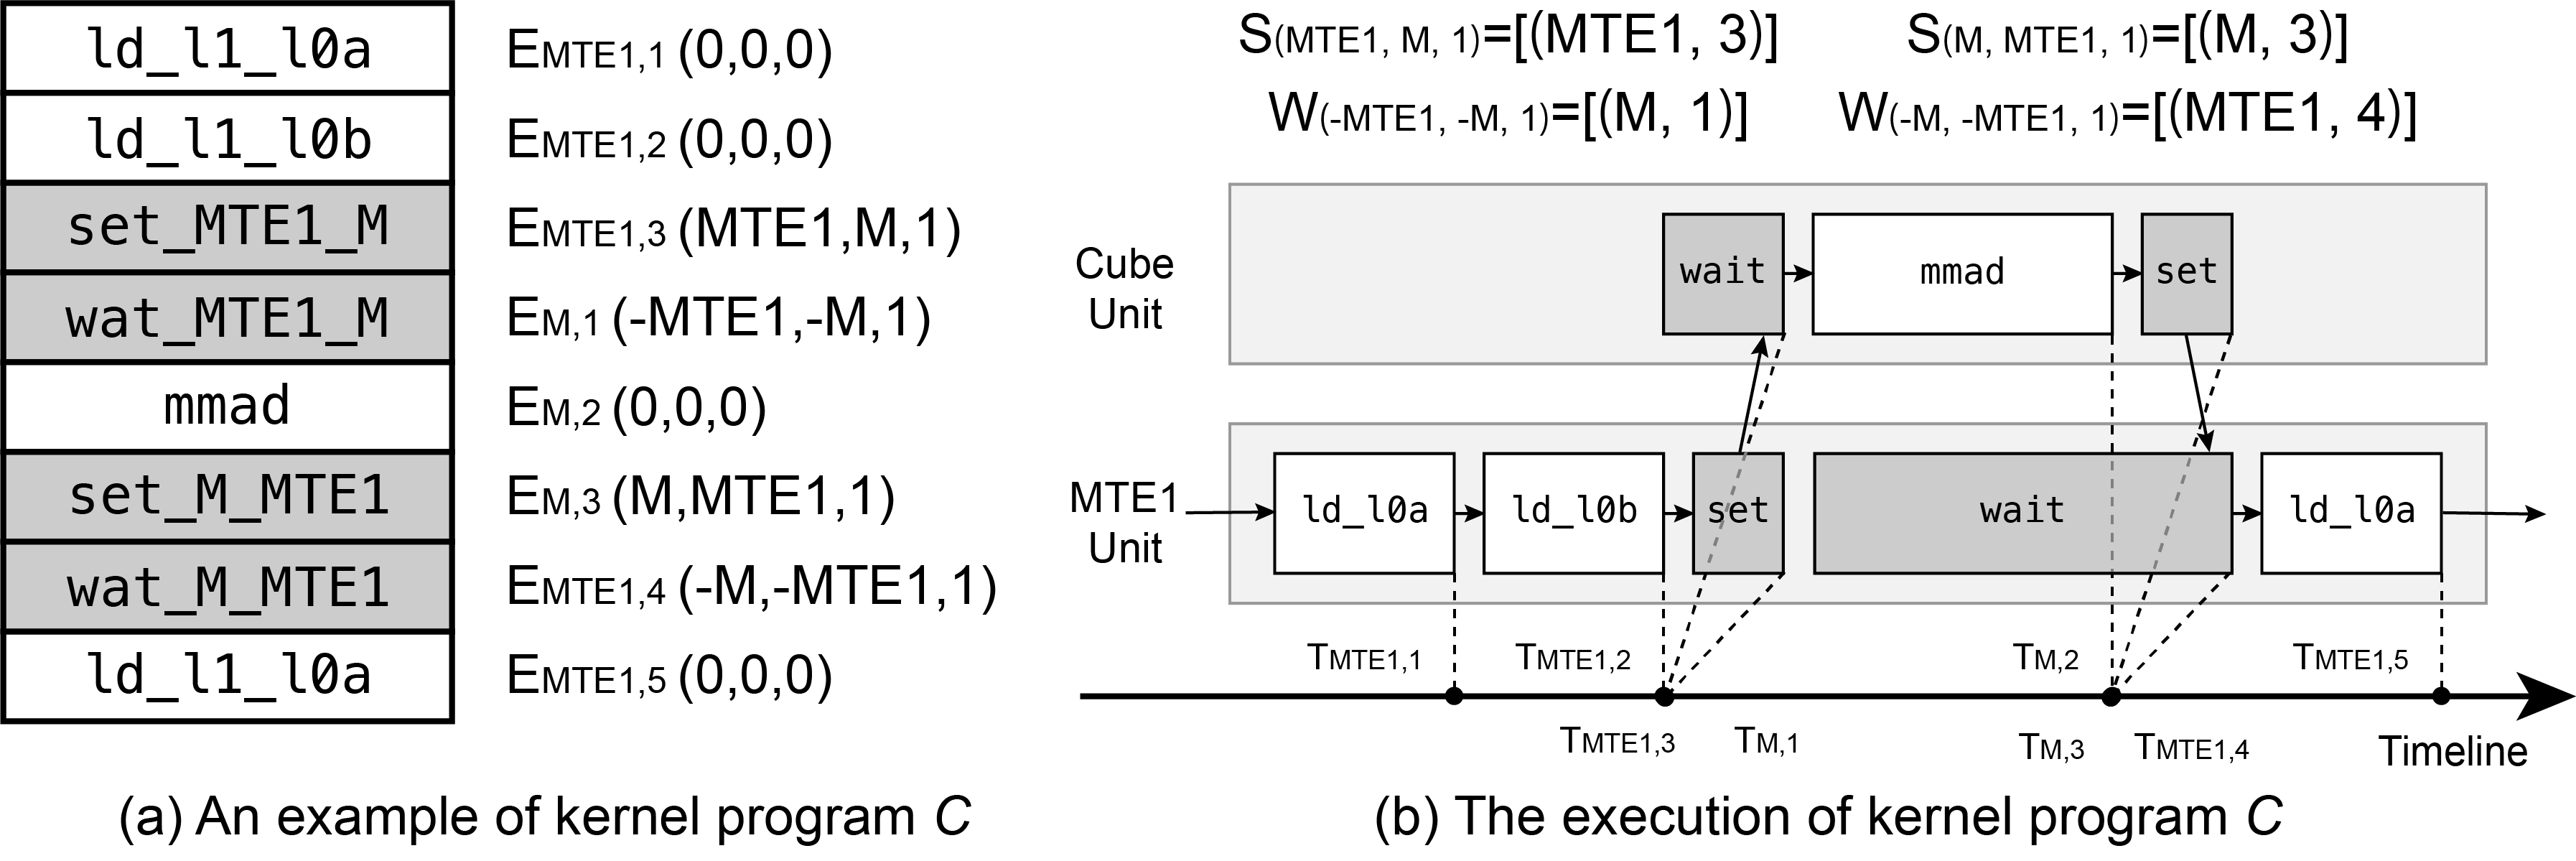
\includegraphics[scale=0.39]{figures/modeling.png}}
    \caption{An example of Verrocchio main performance modeling procedure}
    \label{fig:modeling}
\end{figure}

For the normal operations, we set $E_{u, n} = (0, 0, 0)$, which means $E_{u, n}$ is not related to the binary semaphore mechanism. For each normal computation or memory operation $E_{u, n}$, we first compute the corresponding static execution period $P_{u, n}$ to quantify how long the $E_{u, n}$ could occupy the Unit $u$. In general,  $P_{u, n}$ is computed as shown in Alg. \ref{alg:model} line 4. According to the FIFO policy, the incidence of $E_{u, n}$ should be immediately after the death of $E_{u, n-1}$. Hence, we compute the death $T_{u, n}$ of $E_{u, n}$ as the sum of the last death time $T_{u, n-1}$ on the same Unit $u$ and the event execution period $P_{u, n}$, as shown in Alg. \ref{alg:model} line 5.

\subsubsection{Set Flag Operations}

For the Set Flag operations, we set $E_{u, n} > (0, 0, 0)$. For the example in Fig. \ref{fig:modeling} (a), the instruction \verb|set_MTE1_M| is converted to $E_{MTE1, 3} = (MTE1, M, 1)$, which means the MTE1 Unit has finished its work, and the Cube Unit should terminate its corresponding Wait Flag operation and continue its next operation with Register 1. Since the Set Flag operations do not suspend or finish any workloads, the death time $T_{u, n}$ equals the last death time $T_{u, n-1}$.

Before the Main Performance Modeling Procedure, we create and maintain an array $S_{E_{u, n}}$ to store the Set Flag operations with the subscript of the 3-tuple $(u_{a}, u_{b}, r)$. We store the 2-tuple $(u, n)$ of $E_{u, n}$, the identification of the Set Flag operation. We have the definition of $S_{E_{u, n}}$ shown below:

\begin{equation}
\begin{aligned}
S_{E_{u_{1}, n_{1}}} = & S_{E_{u_{2}, n_{2}}} = S_{(u_{a}, u_{b}, r)} = \langle (u_{1}, n_{1}), (u_{2}, n_{2}), ... \rangle \\
& \forall E_{u, n} > (0, 0, 0), n_{i} < n_{j}, \forall i < j
\end{aligned}
\end{equation}

where the array $S_{E_{u, n}}$ is sorted according to the operation order number $n$.

\subsubsection{Wait Flag Operations}

For the Wait Flag operations, we set $E_{u, n} < (0, 0, 0)$, which is symmetric to the Set Flag operation definition. For the example in Fig. \ref{fig:modeling} (a), the instruction \verb|wait_MTE1_M| is converted to $E_{M, 1} = (-MTE1, -M, -1)$. We also create and maintain an array $W_{E_{u, n}}$ to store the 2-tuple $(u, n)$, as shown below:

\begin{equation}
\begin{aligned}
W_{E_{u_{1}, n_{1}}} = W_{E_{u_{2}, n_{2}}} = & W_{(-u_{a}, -u_{b}, -r)} = \langle (u_{1}, n_{1}), (u_{2}, n_{2}), ... \rangle \\
\forall E_{u, n} < & (0, 0, 0), n_{i} < n_{j}, \forall i < j
\end{aligned}
\end{equation}

For a Wait Flag operation $E_{u, n}$, its corresponding Set Flag operation $E_{u^{\prime}, n^{\prime}}$ must exist, where $E_{u, n} = - E_{u^{\prime}, n^{\prime}}$, as shown in Alg. \ref{alg:model} line 9. The array $S$ and $W$ are used to locate the related Set Flag and Wait Flag operation pair. Since DaVinci Cores have no memory heap or stack structure but only registers to store the semaphores, the Wait Flag operation order number in $W_{E_{u, n}}$ equals the order number of its corresponding Set Flag operation in $S_{E_{u^{\prime}, n^{\prime}}}$. We introduce a function $Index(x, Array)$ to return the position of $x$ in an array $Array$ without duplicated elements, then we have the relation:

\begin{equation}
Index((u, n), W_{E_{u, n}}) = 
    Index((u^{\prime}, n^{\prime}), S_{E_{u^{\prime}, n^{\prime}}}) = 
    Index((u^{\prime}, n^{\prime}), S_{- E_{u, n}})
\end{equation}

Hence, we have:

\begin{equation}
(u^{\prime}, n^{\prime}) = S_{- E_{u, n}}[Index((u, n), W_{E_{u, n}})]
\end{equation}

Since a Wait Flag operation blocks the Unit until the corresponding Set Flag operation is done, the death time of the Wait Flag operation equals the Set Flag operation death time. For the example in Fig. \ref{fig:modeling} (b), we compute $T_{M, 1}$ as follows:

\begin{equation}
\label{eq:wait}
T_{M, 1} = T_{S_{-E_{M, 1}}[Index((M, 1), W_{E_{M, 1}})]}
    = T_{S_{(MTE1, M, 1)}[0]}
    = T_{MTE1, 3}
\end{equation}

\subsubsection{Bandwidth Contention Updating}

As we discussed, the bandwidth contention of the Interconnect Bus influences the performance of the MTE2 and MTE3 Units significantly. The runtime behaviors we expose in Sec. \ref{sec:runtime} show that each time the two Units start to run concurrently, the contention occurs, and the related bandwidth changes; when either of the Units finishes, the contention ends, and the Units regain the original bandwidth. For the example in Fig. \ref{fig:contention} (a), at $T_{MTE3, 1}$, when the MTE3 starts to execute the instruction \verb|ld_ub_to_gm|, the contention begins; when the MTE2 Unit finishes its work at $T_{MTE2, 1}$, the contention is finished. Therefore, the contention status changes at the event death time. Verrocchio checks whether a contention appears or disappears when an event is finished to update the death time of the related events.

\begin{figure}[tbp]
    \centering{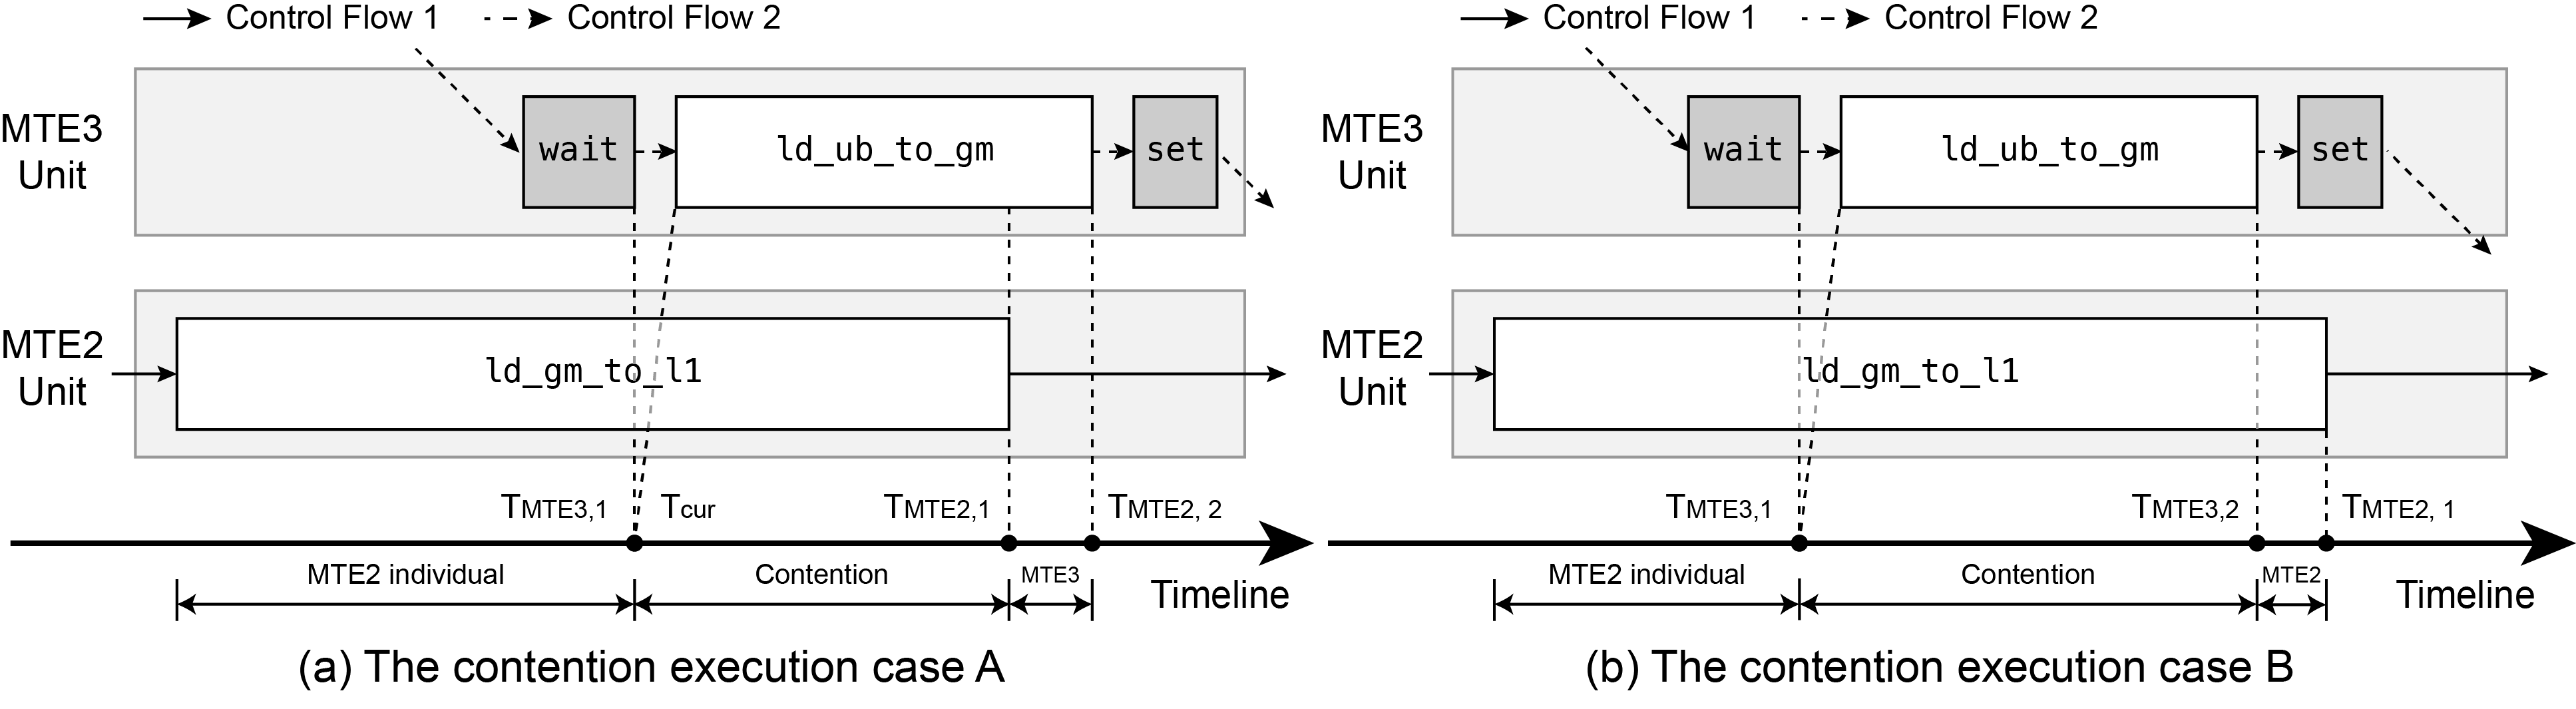
\includegraphics[scale=0.37]{figures/contention.png}}
    \caption{Examples of Verrocchio contention execution}
    \label{fig:contention}
\end{figure}

We first compute the left data size of the event, which is influenced by the contention status change. For an event $E_{u, n}$, we compute the left data size as shown below:

\begin{equation}
Ds^{\prime}_{u, n} = Ds_{u, n} \times \frac{T_{u, n} - T_{cur}}{P_{u, n}}
\end{equation}

where $T_{cur}$ is the current global time, also the death time of the latest event triggering the bandwidth contention, e.g., $T_{MTE3, 1} = T_{cur}$ in Fig. \ref{fig:contention} (a), $Ds^{\prime}_{u, n}$ is the data size left for the new contention status. Then we update the event death time as follows:

\begin{equation}
T^{\prime}_{u, n} = T_{cur} + Ds^{\prime}_{u,n}\;/\;Th^{\prime}_{u}
\end{equation}

where $Th^{\prime}_{u}$ is the bandwidth of the Unit $u$ at the new contention status, $T^{\prime}_{u, n}$ is the new death time. For $Th^{\prime}_{u}$, we strictly follow our conclusions in Sec. \ref{sec:bw_sr_res}, where multiple Units equally share the bandwidth. The potential executions with a contention are divided into two cases shown in Fig. \ref{fig:contention}, based on the relationship of the two events' execution period. For the case in Fig. \ref{fig:contention} (a), both units suffer one contention status change; for Fig. \ref{fig:contention} (b), one unit suffers two contention status changes, experiencing the three-segment polyline of bandwidths discussed in Sec. \ref{sec:runtime}. 

\subsection{Multi-core Execution Performance Modeling \label{sec:multi-core}}

According to our benchmark results, the DaVinci hardware units can be classified into two categories, the one which relies on the independent on-core resources and the other which occupies the Interconnect Bus and causes contentions. For the first category, the throughput $Th_{single}$ of every single core does not change (as a const value $C_{single}$) in the multi-core execution, and the total unit throughput $Th_{total}$ of all cores increases proportionally.

\begin{equation}
\label{eq:first}
Th_{single} = C_{single} \qquad Th_{total} = N \times Th_{single}
\end{equation}

where $N$ is the number of the activated DaVinci Cores. For the second category, as our benchmarks report in Sec. \ref{sec:bw_sr_res}, the throughputs of all single core $Th_{single}$ averagely share the total throughput.

\begin{equation}
\label{eq:second}
Th_{single} = \frac{Th_{total}}{N} \qquad Th_{total} = C_{total} 
\end{equation}

Like most multi-core accelerators, we assume that multi-core DaVinci processors continue to adopt the SIMD execution model, which means the programs are tiled and distributed to multiple cores. We focus on a general normal computation or memory operation $E_{u, n}$, submitted to multiple DaVinci Cores, as shown in Fig. \ref{fig:multi-core}, where each bar is a tile of $E_{u, n}$, e.g. $Tile_{1}$, $Tile_{2}$. To model the differences in the $E_{u, n}$ incident time $T_{u, n_{inc}}$ in all DaVinci Cores (e.g. $T_{inc_{2}} - T_{inc_{1}}$), we introduce $\delta_{t}$, which can be measured in our benchmarks. It represents the average interval between the two nearest incident times among all DaVince Cores.

For each tile of $E_{u, n}$ among all DaVinci Cores, the workloads (data sizes) $Ds_{single}$ are the same. Because of $\delta_{t}$, the tile of $E_{u, n}$ on each core shows a stepped execution pattern with a start-up time. The execution period $P_{u, n}$ of $E_{u, n}$ for case (a) in Fig. \ref{fig:multi-core} is calculated as below:

\begin{figure}[tbp]
    \centering{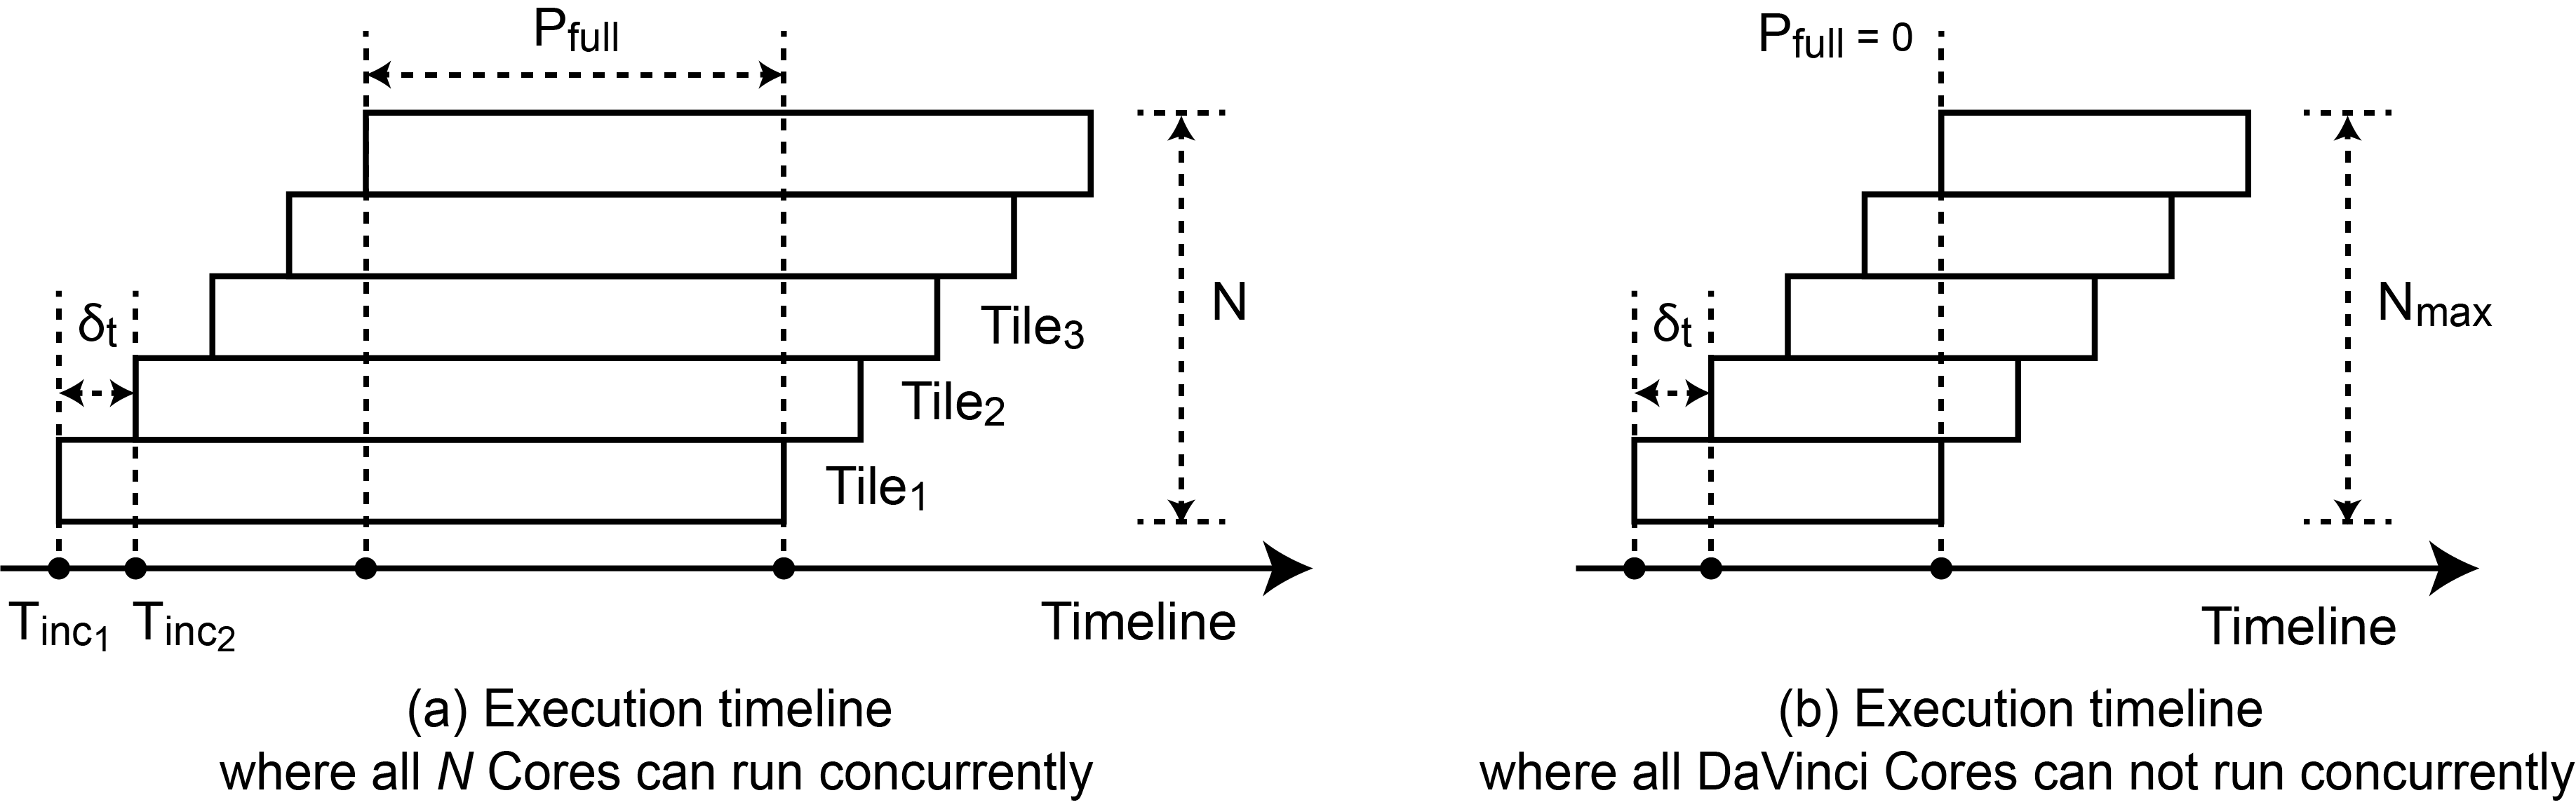
\includegraphics[scale=0.38]{figures/multicore.png}}
    \caption{
    Execution timeline of $E_{u, n}$, which is tiled and submitted to multiple DaVinci Cores}
    \label{fig:multi-core}
    \end{figure}    

\begin{equation}
P_{u, n} = 2 (N - 1) \delta_{t} + P_{full}
\end{equation}

where $P_{full}$ is the period when all the cores are running concurrently. The execution period $P_{u, n}$ of $E_{u, n}$ for case (b) is calculated as below:

\begin{equation}
P_{u, n} = 2 (N_{max} - 1) \delta_{t}
\end{equation}

where $N_{max}$ is the maximized all-busy core number for the event $E_{u, n}$. Then, to calculate $P_{u, n}$, we must determine $P_{full}$ and $N_{max}$ first. For the first category of the units, which relies on the independent on-core resources only, we have Eq. \ref{eq:first_eq} for the case (a) in Fig. \ref{fig:multi-core}:

\begin{equation}
\label{eq:first_eq}
\begin{aligned}
    2 Th_{single} \delta_{t} \times \sum_{i=1}^{N-1}{i} + & N \times Th_{single} P_{full} = N \times Ds_{single} \\
    \implies P_{full} = & \frac{Ds_{single} - (N - 1) Th_{single} \delta_{t}}{Th_{single}} 
\end{aligned}
\end{equation}

Fig. \ref{fig:multi-core} shows that, the condition converting the case (a) to the case (b) is $P_{full} = 0$, which means that all DaVinci Cores cannot run concurrently and then the core number $N$ is $N_{max}$. Then we have the relation shown below:

\begin{equation}
P_{full} = \frac{Ds_{single} - (N_{max} - 1) Th_{single} \delta_{t}}{Th_{single}} = 0 \implies
N_{max} = \frac{Ds_{single}}{Th_{single} \delta_{t}} + 1
\end{equation}

We follow a similar idea for the second category of units as for the first category units. Hence, we list the equation below:

\begin{equation}
\label{eq:second_eq}
    \begin{aligned}
    2 Th_{total} \delta_{t} \times (N - 1) + Th_{total} P_{full} & = N \times Ds_{single} \\
    P_{full} = \frac{N Ds_{single} - 2 (N - 1) Th_{total} \delta_{t}}{Th_{total}}
    \  
    N_{max} & = \frac{2 Th_{total} \delta_{t}}{2 Th_{total} \delta_{t} - Ds_{single}}
    \end{aligned}
\end{equation}

The Ascend 310 processors are the simplest DaVinci architecture processors and have two DaVinci Cores, and then we have $N = 2$. According to our benchmark results, as shown in Table \ref{tab:bench}, $\delta_{t} \approx 61 ns$, which is $2.5\%$ of the kernel launch time and can be ignored. Hence, in the double-core execution, the total time can be simplified to $P_{u, n} = P_{full} = Ds_{single} / Th_{single}$ for the first category of units or $P_{u, n} = N \times Ds_{single} / Th_{total}$ for the second category.

% Evaluation Section

\section{Evaluation}

This section evaluates the accuracy of Verrocchio. We first implement several basic kernels for the accuracy evaluations. Then as a complicated test case and a demonstration of the usage of Verrocchio, we show a matrix multiplication optimizing process guided by Verrocchio. All the experiment results are collected by Huawei's official profiler on the Ascend 310 processor (two DaVinci Cores) with Huawei Kunpeng 920 2.6GHz CPU equipped.

\subsection{Sample Kernel Evaluation}

Table \ref{tab:kernel_type} lists the sample kernels we implement for evaluations. The cases include memory transfers, single computations, and several basic applications. We evaluate the accuracy results for both single-core and double-core situations. Fig. \ref{fig:tiny} illustrates the evaluated error rate results for each case.

Generally, Verrocchio reports high accuracy results. For the single-core execution, the average error rate is $2.62\%$; for the double-core execution, the result is $2.30\%$. The error rates among all cases do not show a system error but are randomly scattered around the baseline. The single-core kernel \textit{mte1B} reports the maximum error rate of $7.33\%$. On the other hand, for the double-core execution, \textit{mte1B} reports a much lower error rate of $3.14\%$. Since the MTE1 Unit is the independent on-core unit we discussed in Sec. \ref{sec:multi-core}, which does not suffer the performance loss in the multi-core execution, \textit{mte1B} is expected to show similar error rates in the two situations. Therefore, the practical results suggest that the MTE1 Unit is not stable as other independent on-core units, which may require deeper analyses. In addition, we observe that the error rates of the Application kernels and the Memory Transfer kernels are higher than the Single Operation kernels, which indicates that the memory transfers, especially between the on-core buffers and the external storage, are the main prediction error sources of Verrocchio.

\begin{figure}[tbp]
    \centering{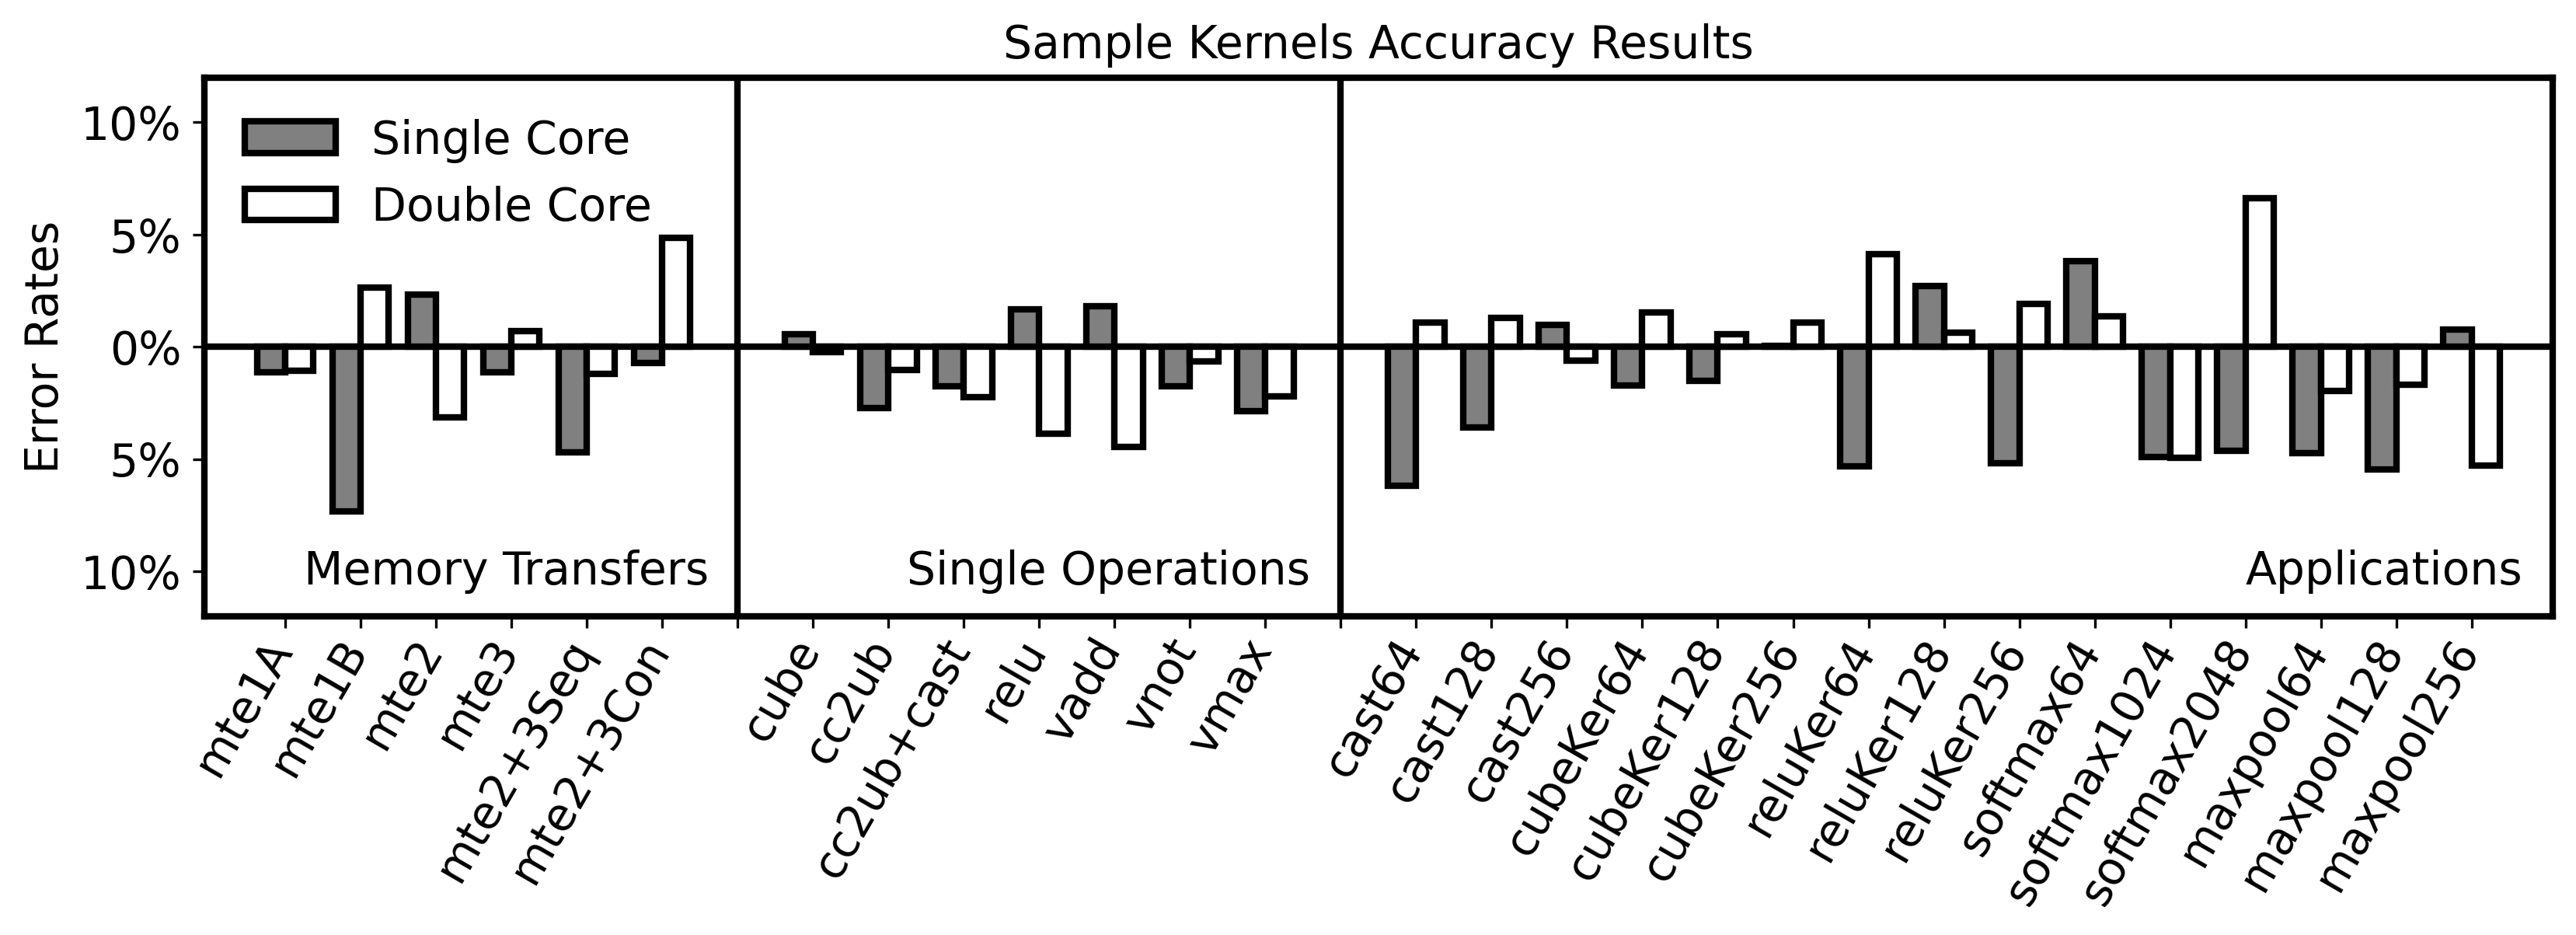
\includegraphics[scale=0.48]{figures/tiny_kernels.png}}
    \captionsetup{justification=centering}
    \caption{The Verrocchio error rate results for sample kernels}
    \label{fig:tiny}
    \end{figure}

\begin{table}[t]
    \caption{Verrocchio sample kernels for accuracy evaluation}
    \label{tab:kernel_type}
    \begin{center}
    
    \scalebox{0.72}{
        \begin{tabular}{c|c|c}    
        \toprule[1pt]
        \textbf{Categories} & \textbf{Kernel Name} & \textbf{Description} \\
        \midrule[0.5pt]

        \multirow{6}*{Memory transfers} & mte1A & Transfer data from L1 Buffer to L0A Buffer \\
        ~ & mte1B & Transfer data from L1 Buffer to L0B Buffer \\
        ~ & mte2 & Transfer data from external storage to L1 Buffer \\
        ~ & mte3 & Transfer data from Unified Buffer to external storage\\
        ~ & mte2+3Seq & MTE2 and MTE3 Units execute sequentially \\
        ~ & mte2+3Con & MTE2 and MTE3 Units execute concurrently \\
        \midrule[0.5pt]
        \multirow{7}*{Single computations} & cube & Do a matrix multiplication w/ Cube Unit\\
        ~ & cc2ub & Transfer from L0C Buffer to Unified Buffer w/ Vector Unit \\
        ~ & cc2ub+cast & Same as above plus type conversion\\
        ~ & relu & ReLU activation function \\
        ~ & vadd & Vectorized addition\\
        ~ & vnot & Vectorized boolean NOT operation\\
        ~ & vmax & Vectorized element-wise Max operation\\
        \midrule[0.5pt]
        \multirow{5}*{\makecell[c]{Applications \\ (Full kernels \\ with I/O)}} & castXxx & Type conversion operator \\
        ~ & cubeKerXxx & Matrix multiplication operator without tiling \\
        ~ & reluKerXxx & ReLU activation operator\\
        ~ & softmaxXxx & Softmax operator\\
        ~ & maxpoolXxx & MaxPooling operator\\
    
        \bottomrule[1pt]
        \end{tabular}
    }
\end{center}
\end{table}
    
\subsection{Matrix Multiplication Optimizing Process}

This section demonstrates an optimizing process of matrix multiplication with Verrocchio, one of the most significant applications for AI processors.

\begin{algorithm}[tbp]
    \caption{Target Improved Matrix Multiplication}
    \label{alg:mat}
    
    \SetKwInOut{Input}{input}
    \SetKwInOut{Output}{output}
    
    \Input{
        matrix \textbf{A}, \textbf{B} of size ($\textit{m} \times \textit{k}$), ($\textit{k} \times \textit{n}$) \\
        % matrix  of size  \\
        tiling parameter \textit{mTiles}, \textit{kTiles}, \textit{nTiles}, \textit{bNum}
    }
        
    \Output{
        matrix \textbf{C} of size ($\textit{m} \times \textit{n}$)
    }
    \BlankLine
    
    % \CommentSty{\# Compute the size of each tile} \\
    (\textit{mSlice}, \textit{kSlice}, \textit{nSlice}) $\leftarrow$ (\textit{m}, \textit{k}, \textit{n}) $/$ 
        (\textit{mTiles}, \textit{kTiles}, \textit{nTiles}) \\
    % \CommentSty{\# Direction Order M $\rightarrow$ N $\rightarrow$ K} \\
    \For{$i \leftarrow 0, j \leftarrow 0$ \KwTo \textit{mTiles}, \textit{nTiles}}{
            \For{$l \leftarrow 0, bf \leftarrow 0$ \KwTo \textit{kTiles} $/$ \textit{bNum}, \textit{bNum}}{
                    \If{$j = 0$}{
                        load \textbf{A} tile \emph{$mSlice \times kSlice$} to \textit{L1} from \textit{External} \tcp*{MTE2}
                    }
                    load \textbf{A} tile \emph{$mSlice \times kSlice$} to \textit{L0A} from \textit{L1} 
                    \tcp*{MTE1}
                    
                    \If{$i = 0$}{
                        load \textbf{B} tile \emph{$kSlice \times nSlice$} to \textit{L1} from \textit{External} \tcp*{MTE2}
                    }
                    load \textbf{B} tile \emph{$kSlice \times nSlice$} to \textit{L0B} from \textit{L1} 
                    \tcp*{MTE1}
                    do matrix multiplication of \textbf{A} tile $\times$ \textbf{B} tile to \textit{L0C} 
                    \tcp*{Cube}
            }
            % \CommentSty{\# Done the K direction} \\
            load \textbf{C} tile \emph{$mSlice \times nSlice$} to \textit{UB} from \textit{L0C} 
            \tcp*{Vector}
            load \textbf{C} tile \emph{$mSlice \times nSlice$} to \textit{External} from \textit{UB} 
            \tcp*{MTE3}
    }
\end{algorithm}

\subsubsection{Improved Matrix Multiplication and Tiling Parameter Selection}

Alg. \ref{alg:mat} shows the target improved matrix multiplication algorithm for optimization. The matrix multiplications require four tiling parameters, \textit{mTiles}, \textit{kTiles}, \textit{nTiles}, and \textit{bNum}, which represents the tile number from the $m$, $k$, and $n$ directions with the multiple control flow number. 

\begin{figure}[tbp]
    \centering{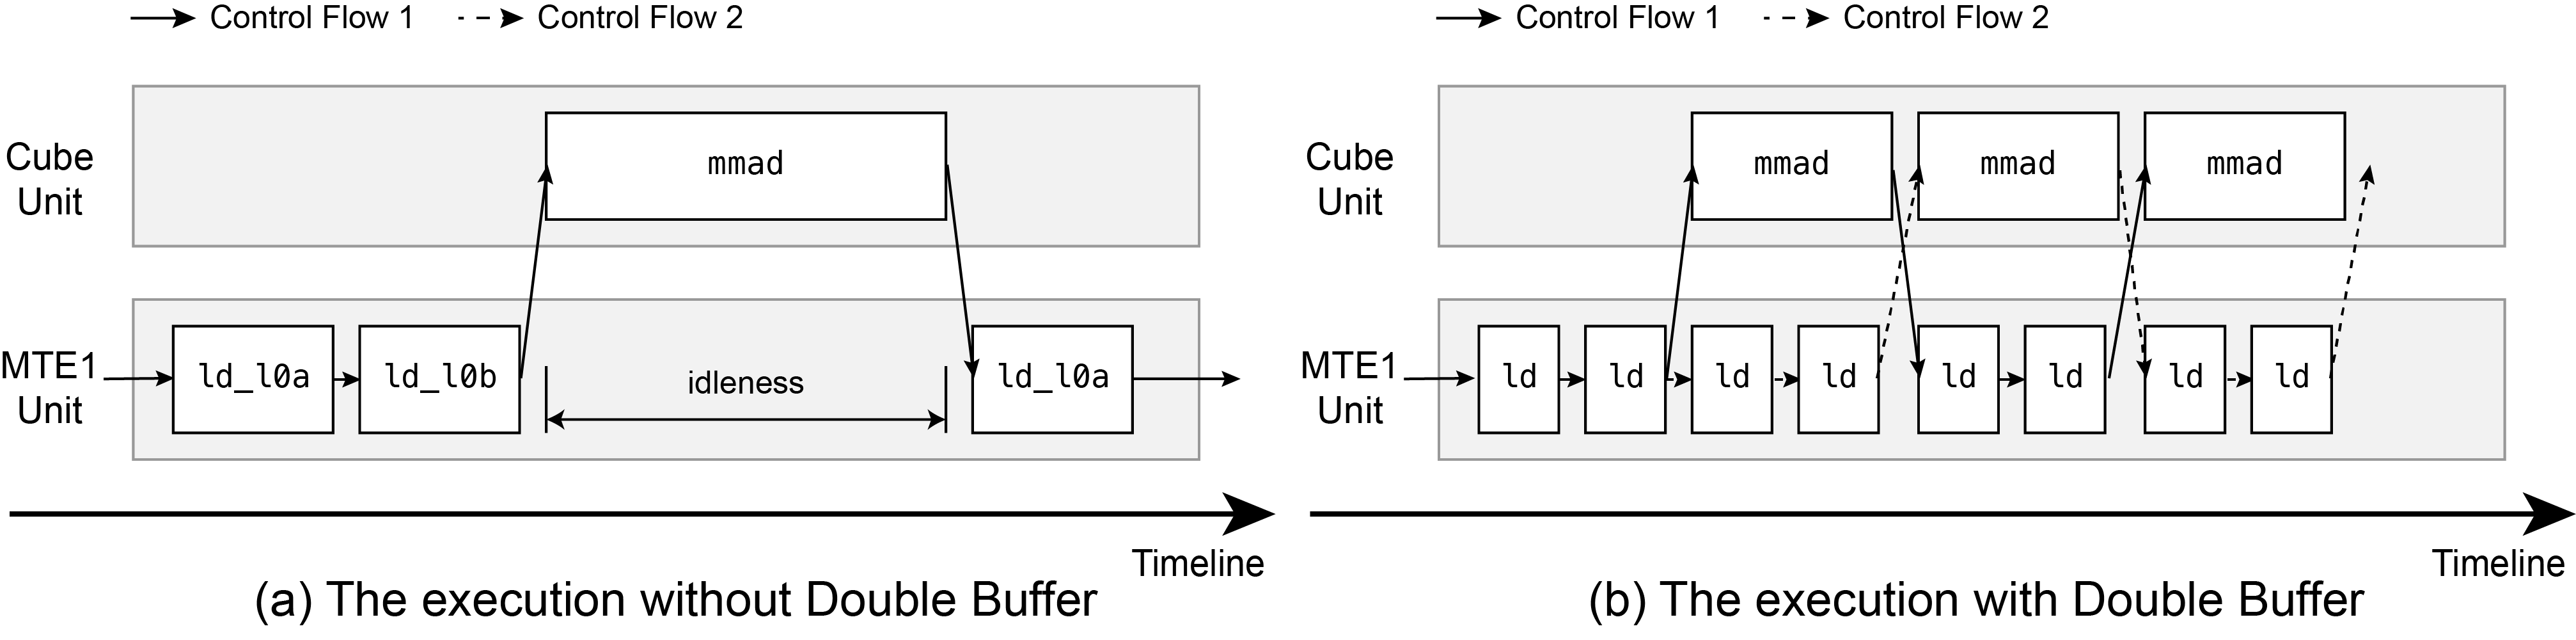
\includegraphics[scale=0.355]{figures/double_buffer.png}}
    \captionsetup{justification=centering}
    \caption{The effect of Double Buffer policy on the execution performance and concurrency}
    \label{fig:doubleb}
    \end{figure}

The matrix multiplication adopts a policy called Double Buffer or Ping-Pong Buffer, shown in Alg. \ref{alg:mat} line 3. DaVinci Core buffers allow reading and writing on different addresses at the same buffer concurrently. Meanwhile, the binary semaphore mechanism allows at most eight independent control flows. Hence, the Double Buffer policy splits the buffers and the operations in half and activates the second control flow. Fig. \ref{fig:doubleb} illustrates how the Double Buffer policy fills the idleness gap of the MTE1 Unit to increase the concurrency and ILP. However, the Double Buffer policy sometimes introduces too much cost and lowers the performance because of the imbalanced execution period.

To formulate an optimization problem, we conduct the tiling parameter selection procedure as a permutation of all four parameters, which are the variables of the problem. The improved matrix multiplication has no further requirements or constraints for the variables, but the tiling numbers must be less than the $16 \times 16 \times 16$ block numbers along the same direction. For each parameter combination in the feasible domain, Verrocchio predicts the execution time and records, which performs the objective function of the optimization problem. To solve the problem, we implement the exhaustive search, the most straightforward solution. Finally, we find the optimized solution as the parameter combination with the least execution time for our matrix multiplication.

\subsubsection{Verrocchio Accuracy Results}

\begin{figure}[tbp]
\centering{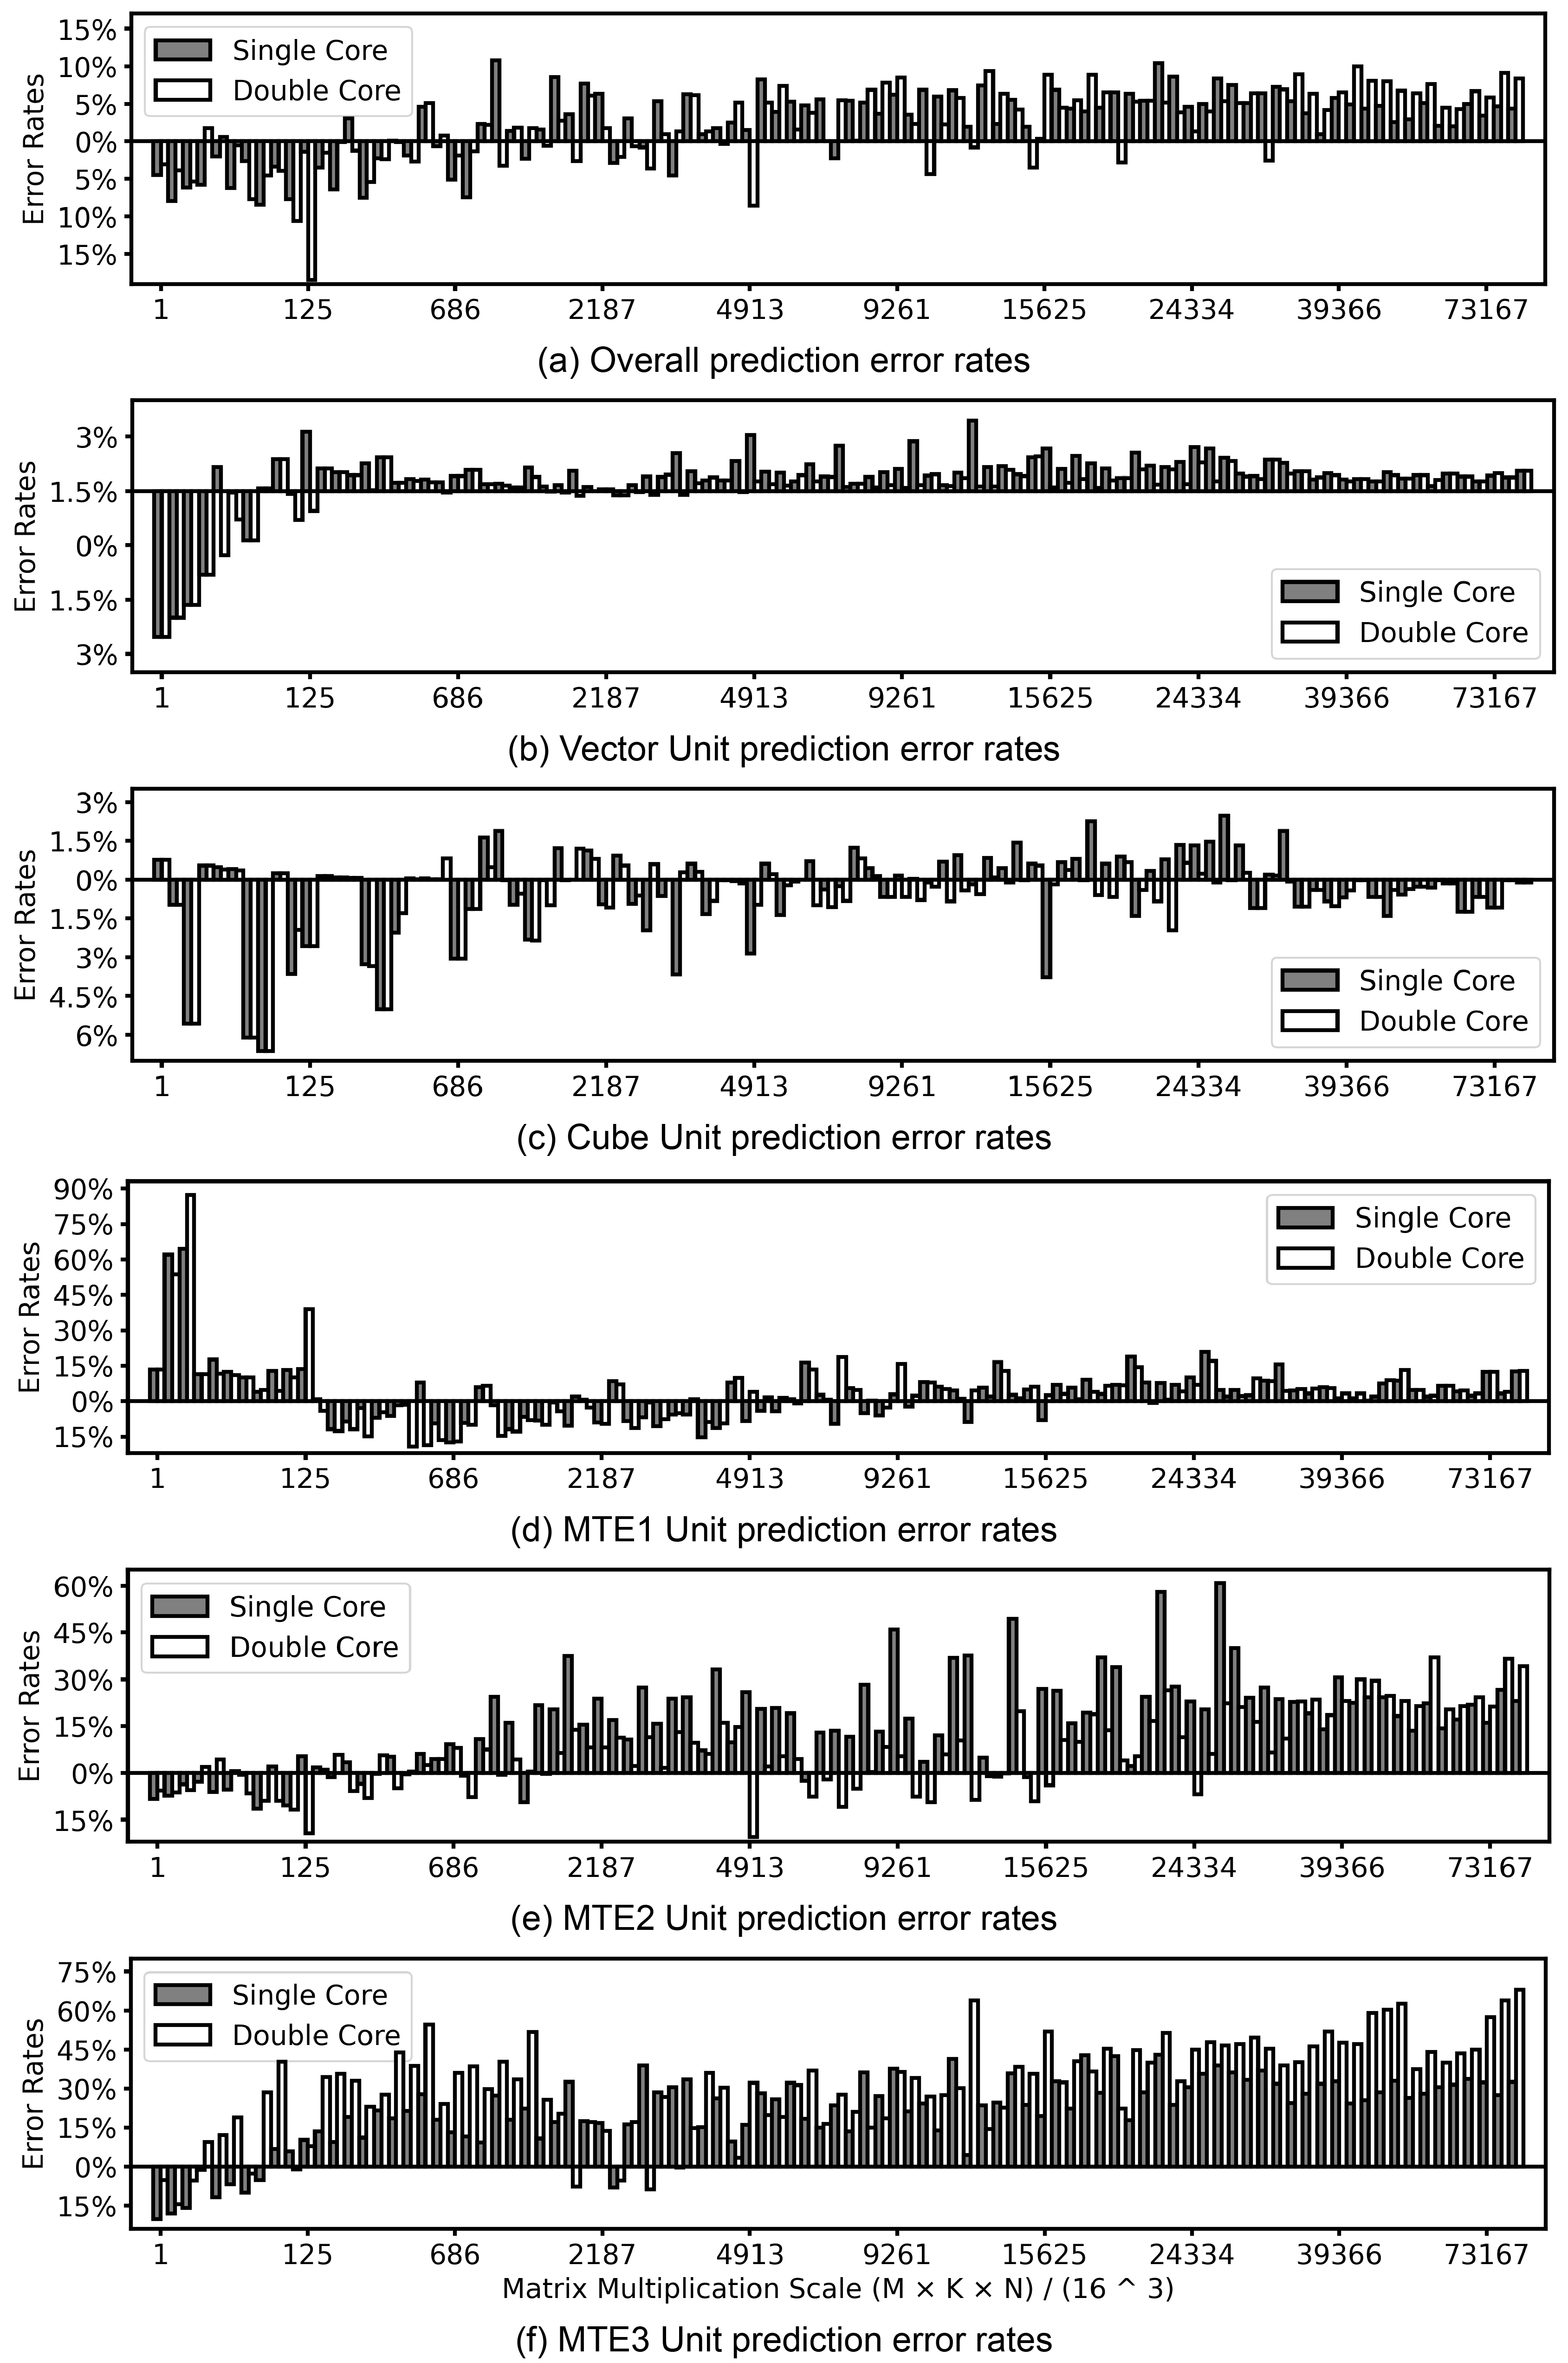
\includegraphics[scale=0.40]{figures/matrixmul.png}}
\captionsetup{justification=centering}
\caption{The Verrocchio error rate results for the improved matrix multiplications}
\label{fig:sim}
\end{figure}

To evaluate the Verrocchio accuracy, we compare our predicted results from Verrocchio with the practical execution time results, which adopt the optimized tiling parameters, as shown in Fig. \ref{fig:sim}. For a better visibility, we define the matrix multiplication scale as the number of the basic blocks operated by the Cube Unit $(m \times k \times n / 16 ^ 3)$. As some matrix multiplications can have the same matrix multiplication scale, we use the average values as the results.

Fig. \ref{fig:sim} (a) shows the total execution time error rates. The average error rate among all test cases is $5.06\%$ for the single-core execution and $5.25\%$ for the double-core execution. The predicted results are lower than the experiment results when the scale is small. One of the potential reasons is that we do not consider the Scalar Unit and the corresponding instructions in Verrocchio. As we discussed in Sec. \ref{sec:ben_des}, the Scalar instructions could block the execution of other units. When the scale gets larger, the effect of the Scalar instructions declines apparently, and the error rates rise above the baseline. When the scale is larger than 5000, the error rates get stable at around 5\%, meaning the prediction of Verrocchio is more accurate and stable in large-scale cases. 

We also show their prediction error rate for each hardware unit separately in the following figures of Fig. \ref{fig:sim}. The Vector Unit and the Cube Unit are well-predicted, reporting the average error rates of $0.69\%$ and $1.17\%$ for the single-core execution, $0.51\%$ and $0.85\%$ for the double-core execution, shown in Fig. \ref{fig:sim} (a) and (b) respectively. The MTE1 Unit performs slightly worse with the average error rates of $9.78\%$ and $9.46\%$. We observe apparent error rates when the scale is small. One of the potential reasons is that the initialization time of the MTE1 instruction is less than other instructions. The MTE2 and MTE3 Units report the worst average error rates of $18.89\%$ and $23.72\%$ for the single-core execution, $14.22\%$ and $33.72\%$ for the double-core execution. Furthermore, the two MTE Units report a system error when the scale is large, where the predicted execution time is always larger than the practical experiment time, especially the MTE3 Unit results. One of the reasons is that, as shown in Fig. \ref{fig:micro_view}, the bus contentions of the MTE Units do not start immediately but wait for the finish of a block. Verrocchio considers all contentions starting at once when the instructions are called, which brings more contentions than the practical execution. In addition, we notice the two MTE Units perform worse in the double-core execution. According to the data collected in Table \ref{tab:bench}, the two DaVinci Cores of the Ascend 310 processors are not synchronized perfectly. Therefore, Verrocchio could bring false contentions in the double-core execution when two respective MTE Units on two cores do not fully overlap.

\subsubsection{Matrix Multiplications Acceleration Results}

\paragraph{Operator Level}

\begin{figure}[tbp]
\centering{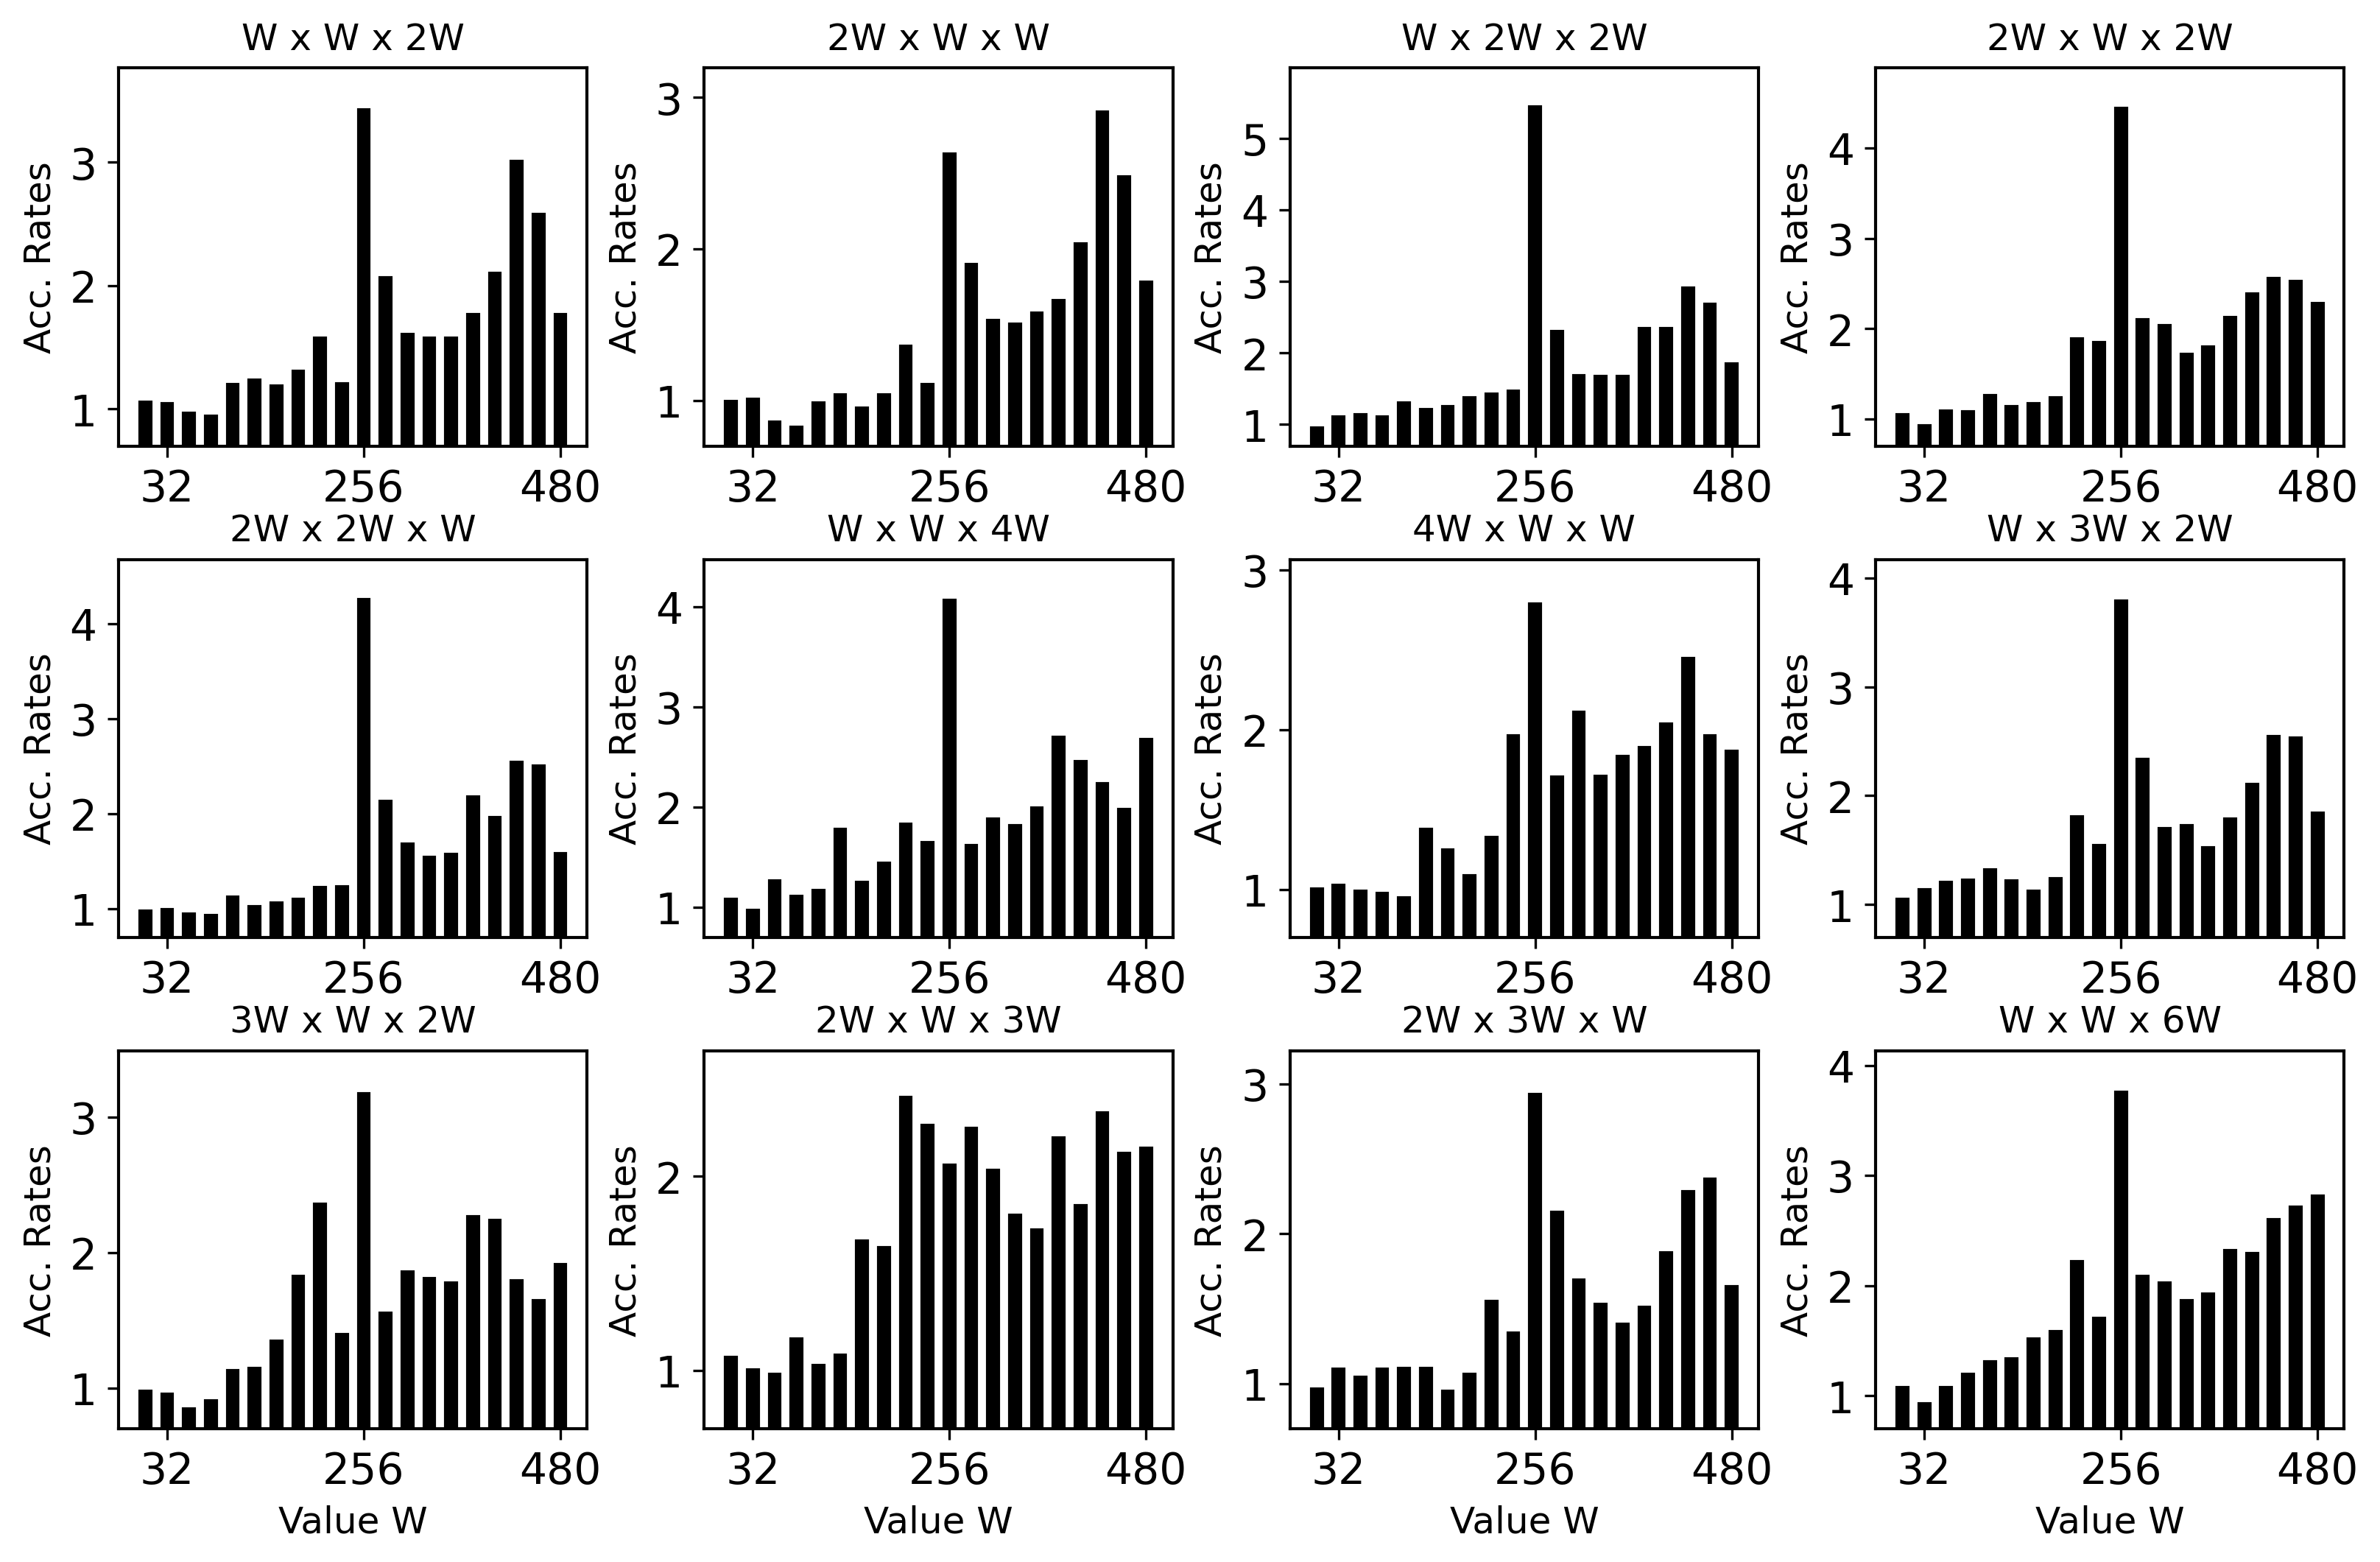
\includegraphics[scale=0.5]{figures/eva.png}}
\caption{Accelerations of the improved matrix multiplication compared with the CANN operators}
\label{fig:eva}
\end{figure}

We compare the improved matrix multiplications with the Huawei CANN operators. As the CANN operators require different logical core numbers, we keep the active core numbers as their respective demands. Our improved matrix multiplication always uses two cores, so we set the core number to two during the experiments of our algorithm. We test matrix multiplications in 12 shapes, from $W \times W \times 2W$ to $W \times W \times 6W$, as shown in Fig. \ref{fig:eva}.

The results show how Verrocchio helps the matrix multiplications to achieve a significant speedup. The improved matrix multiplications achieve an average speedup of 1.70$\times$ among all test cases compared with the Huawei official CANN operators. Generally, the accelerations grow steadily with the increment of the matrix multiplication scale (or value W). For the regular-shaped matrix multiplications like $W \times W \times 2W$, our matrix multiplications show similar performance compared with the CANN operators, where the two approaches follow similar tiling strategies. However, our matrix multiplications perform much better for those irregular-shaped matrix multiplications like $W \times W \times 4W$. The main reason is that the CANN operators abuse the multiple logical cores with inefficient tilings in these irregular-shaped cases, even when the Ascend 310 processors have only two physical cores. Meanwhile, our improved matrix multiplications focus on the two physical DaVinci Cores with the most appropriate and efficient tilings suggested by Verrocchio, which make great improvements.

Furthermore, we plot our matrix multiplications in the roofline model \cite{DBLP:journals/cacm/WilliamsWP09}, as shown in Fig. \ref{fig:roofline}, which considers the Cube Unit FLOPS and the bandwidth between the L0 and L1 Buffer. Compared with the CANN operators, our matrix multiplication algorithm reports a smaller performance gap to the attainable roofline results. The average ratio of the peak hardware performance we achieve is 23.64\%, 2.09X higher than that of the CANN operators. With the increment of the operation intensity, the ratio of our algorithm becomes higher than that of the CANN operators, and finally stops at about 38.78\%, which further proves the better performance in larger scales we observed in Fig. \ref{fig:eva}.

\begin{figure}[tbp]
    \centering{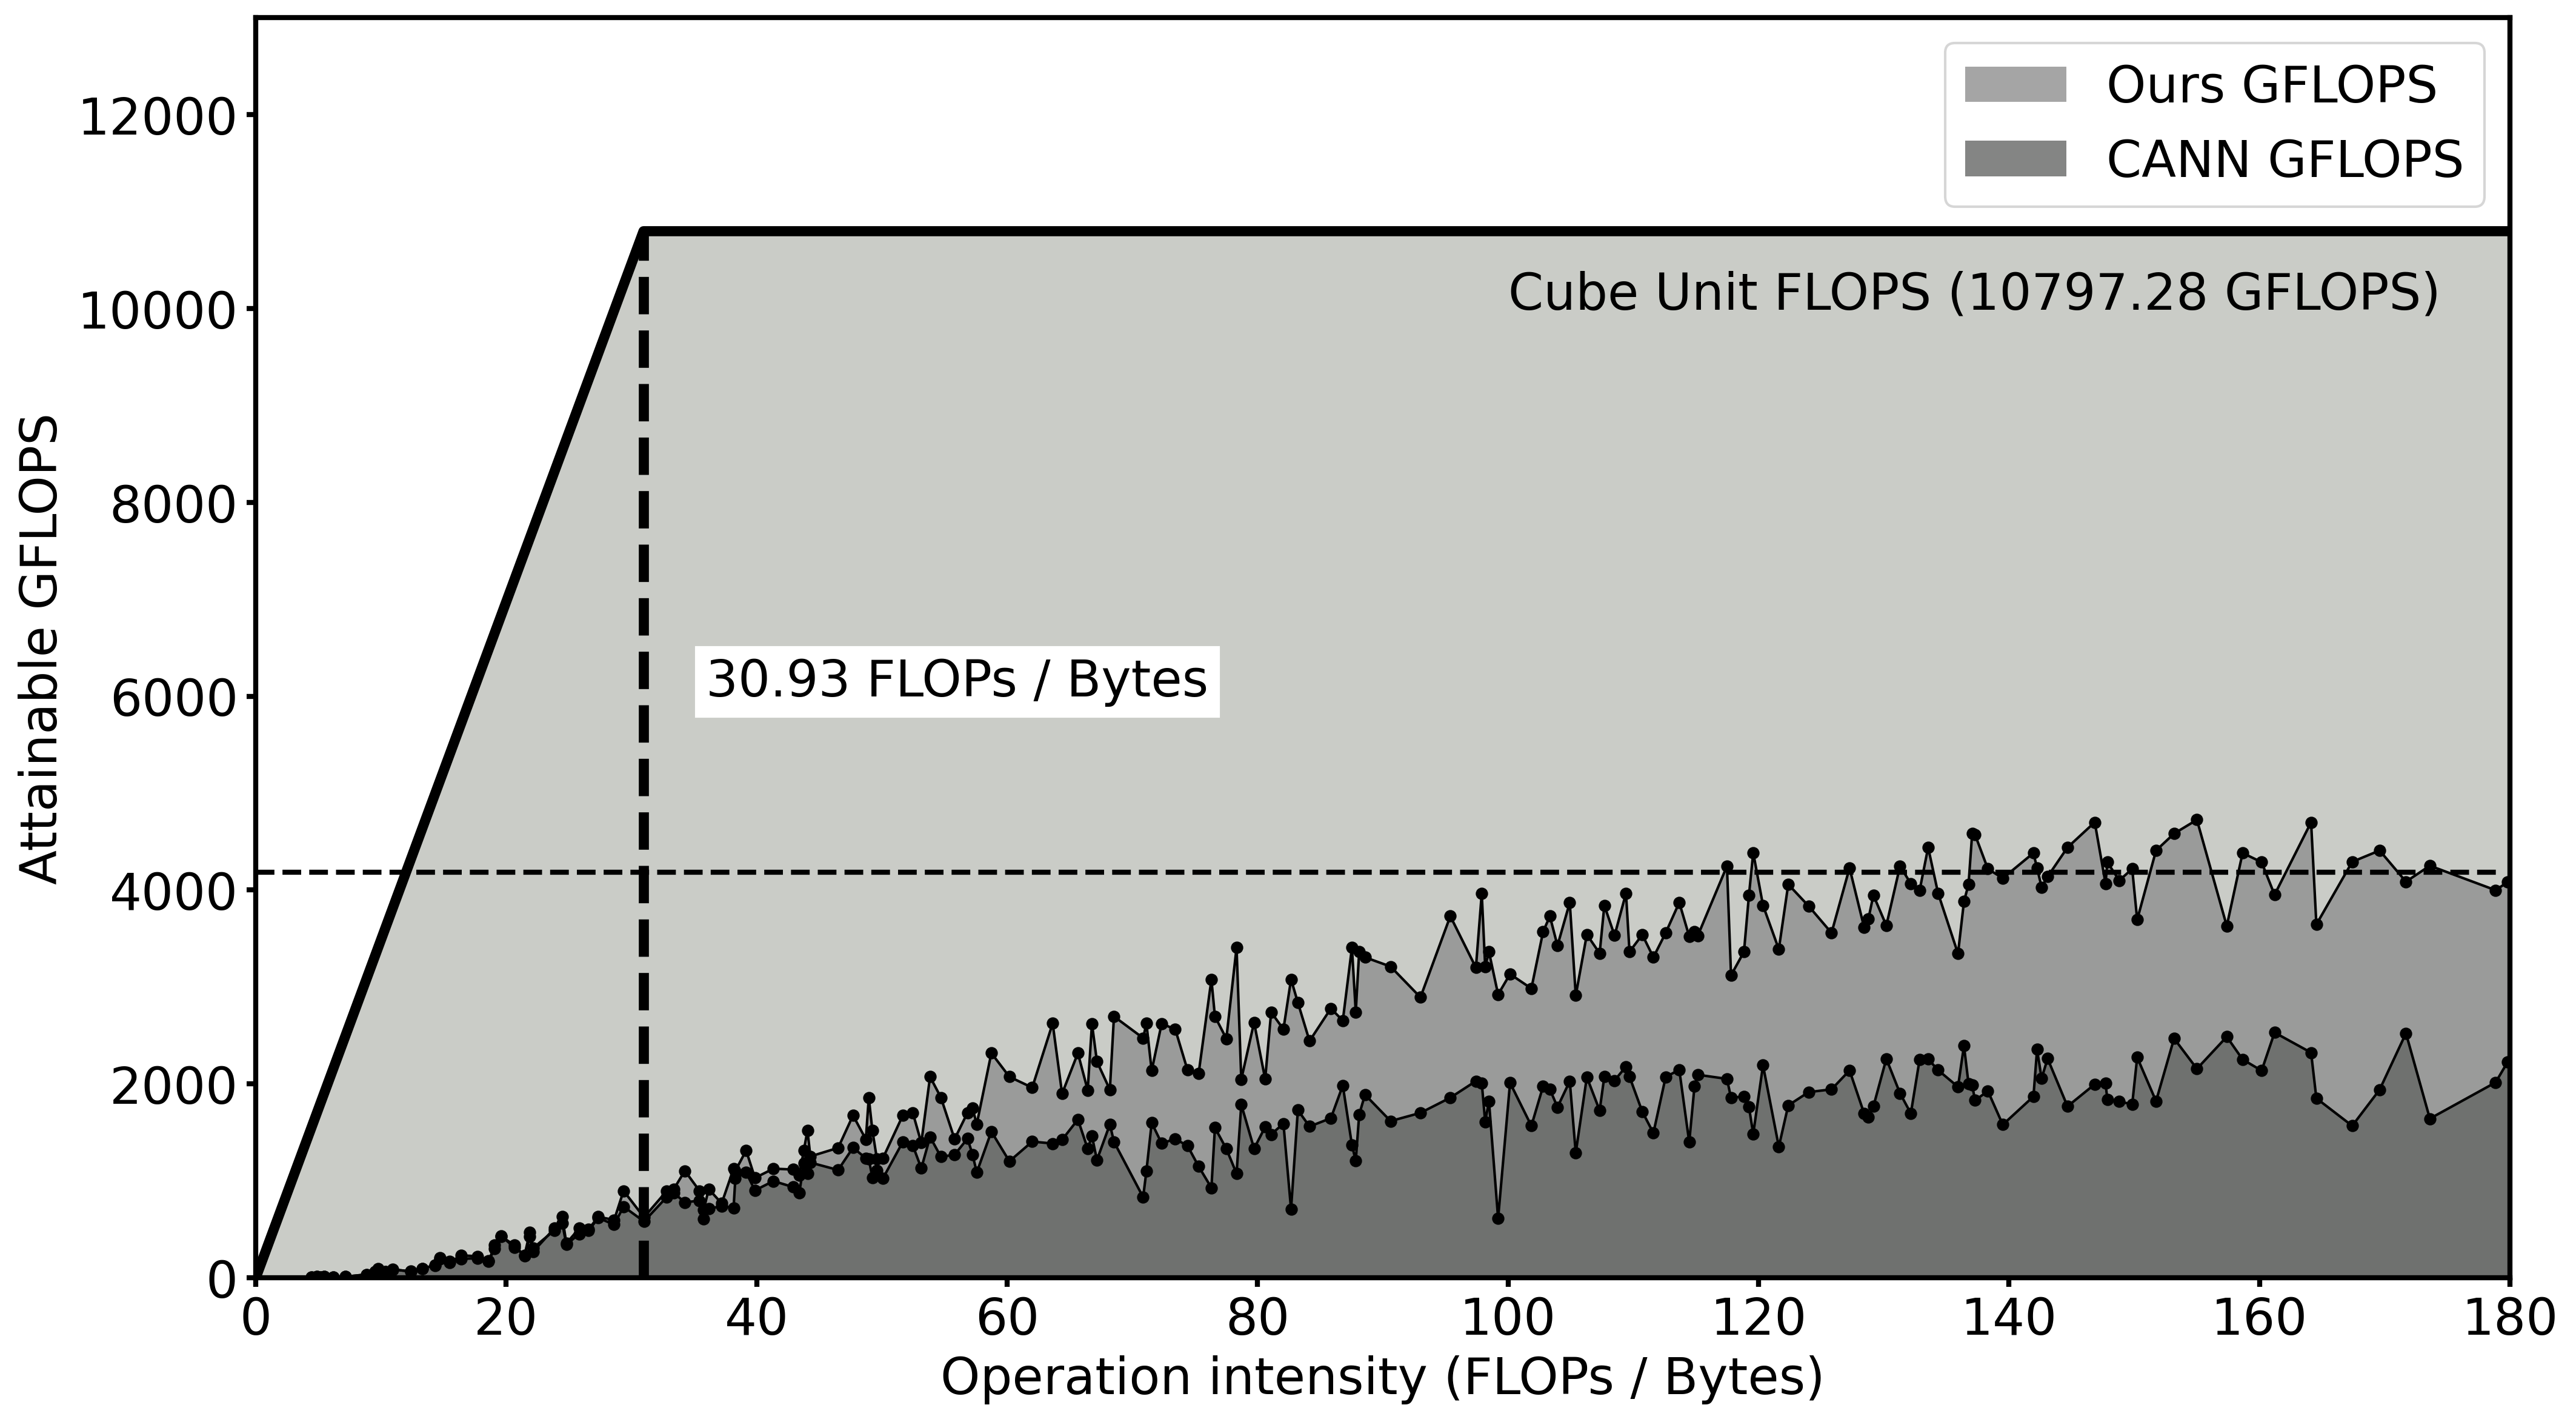
\includegraphics[scale=0.36]{figures/roofline_comp.png}}
    \caption{The roofline model with the matrix multiplication results annotated}
    \label{fig:roofline}
    \end{figure}

\begin{figure}[tbp]
    \centering{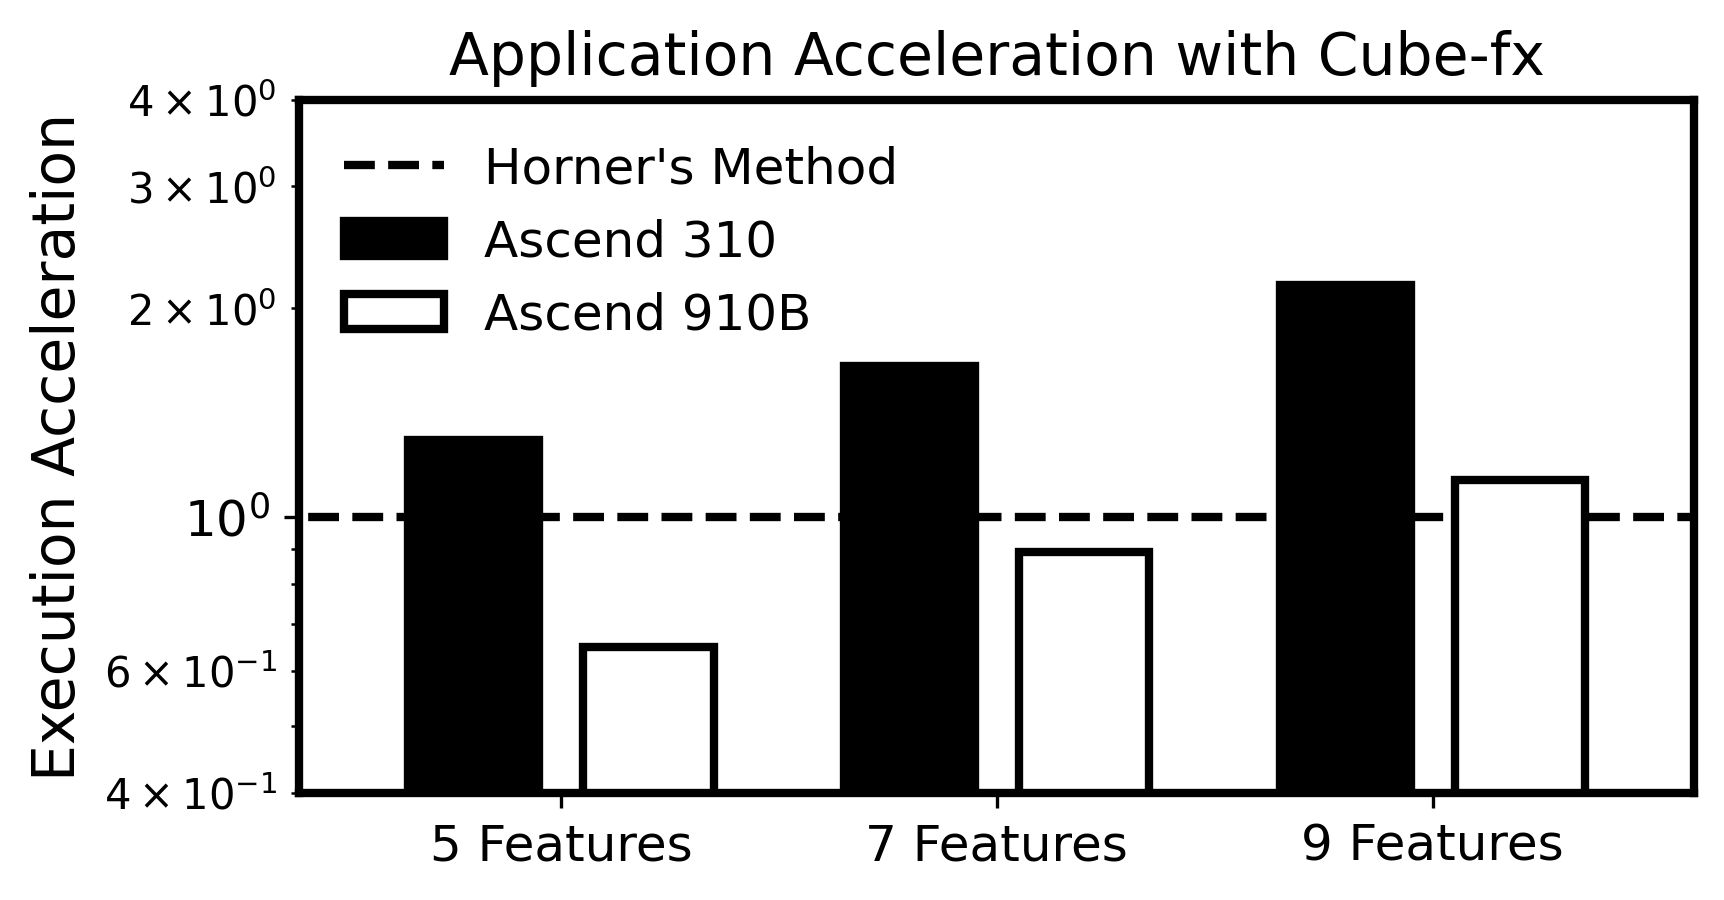
\includegraphics[scale=0.55]{figures/app_acc.png}}
    \caption{The estimation results of the popular DNN applications}
    \label{fig:app_acc}
    \end{figure}
        
\paragraph{Application level}

Currently, executing a DNN model on Ascend 310 processor needs an official ATC offered by Huawei, which converts the Caffe or TensorFlow model to the Huawei custom model. However, Huawei does not offer the structures and formats of the custom model. Hence, we propose an estimated method to evaluate the acceleration brought by the improved matrix multiplications for popular DNN applications. For each layer of a DNN application, we evaluate the total execution time and the Cube Unit execution time. We compute the matrix multiplication scales defined in the last subsection with the collected Cube Unit execution time. Therefore, with the average acceleration rates of the scale, we have an approximate acceleration result of this matrix multiplication operator. By estimating all operators, we have final results of the DNN application \cite{DBLP:conf/cvpr/HeZRS16, DBLP:journals/corr/abs-2004-10934, DBLP:conf/cvpr/SandlerHZZC18, DBLP:conf/nips/KrizhevskySH12, DBLP:conf/naacl/DevlinCLT19}, as shown in Fig. \ref{fig:app_acc}.

Among all evaluation results, AlexNet shows the most significant speedup of 2.18$\times$. The reason is that AlexNet is one of the earliest Convolutional Neural Networks (CNNs) with large Fully Connected (FC) layers. It requires matrix multiplications of a large scale. As we show in the last subsection, the CANN operators perform worse than our operators on a large scale. Generally, the DNN applications report an average speedup of 1.53$\times$. Although YOLO V4 is a complex model, the matrix multiplication scales are not large, reporting the lowest acceleration rate of 1.15$\times$.

\section{Conclusion}

For the first time, we focus on building a performance model, Verrocchio, for Huawei DaVinci AI Cores. The DaVinci Core has complex data paths and distinct working details, which significantly influences the performance and brings a series of modeling challenges. Our discrete-event-based model reports high accuracy for various kernel programs but involves some system errors of the MTE Unit bandwidths, which are caused by the simplification of their runtime behaviors.